\section*{Введение}

В данной лабораторной работе рассматриваются методы спектральной теории графов для анализа сетей. Спектральная теория графов использует собственные числа и собственные векторы матриц, связанных с графами, для решения различных задач анализа сетей.

\textbf{Цель работы:} изучение методов спектральной кластеризации социальных сетей и алгоритма Google PageRank для ранжирования веб-страниц.

\textbf{Задачи:}
\begin{enumerate}
    \item Реализация спектральной кластеризации для выделения сообществ в социальной сети
    \item Изучение алгоритма PageRank и его математических основ
    \item Анализ влияния параметров на качество кластеризации и сходимость алгоритмов
\end{enumerate}

\section*{Задание 1. Кластеризация социальной сети}

\subsection*{Постановка задачи}

Рассматривается социальная сеть, представленная в виде неориентированного графа $G = (V, E)$, где:
\begin{itemize}
    \item $V$ - множество вершин (люди)
    \item $E$ - множество рёбер (отношения дружбы)
\end{itemize}

Задача заключается в выделении сообществ - групп людей, которые в большей степени дружат внутри себя, чем с другими людьми.

\subsection*{Математические основы}

Для спектральной кластеризации используется матрица Лапласа графа:
\begin{equation}
L = D - A
\end{equation}
где:
\begin{itemize}
    \item $D$ - диагональная матрица степеней вершин
    \item $A$ - матрица смежности графа
\end{itemize}

Свойства матрицы Лапласа:
\begin{itemize}
    \item $L$ симметрична и положительно полуопределена
    \item Наименьшее собственное число $\lambda_1 = 0$ с собственным вектором $(1, 1, \ldots, 1)^T$
    \item Количество нулевых собственных чисел равно количеству компонент связности графа
\end{itemize}

\subsection*{Алгоритм спектральной кластеризации}

\begin{enumerate}
    \item Вычисляем матрицу Лапласа $L$
    \item Находим $k$ собственных векторов $v_1, v_2, \ldots, v_k$, соответствующих наименьшим собственным числам
    \item Составляем матрицу $V = [v_1, v_2, \ldots, v_k]$
    \item Применяем алгоритм k-means к строкам матрицы $V$
    \item Кластеризуем вершины графа согласно результатам k-means
\end{enumerate}

\subsection*{Создание тестовой социальной сети}

Создана социальная сеть с 20 вершинами и 42 рёбрами, содержащая три явных сообщества:

\begin{itemize}
    \item Сообщество 1: вершины 1-7 (7 человек)
    \item Сообщество 2: вершины 8-13 (6 человек)
    \item Сообщество 3: вершины 14-20 (7 человек)
\end{itemize}

\begin{figure}[H]
    \centering
    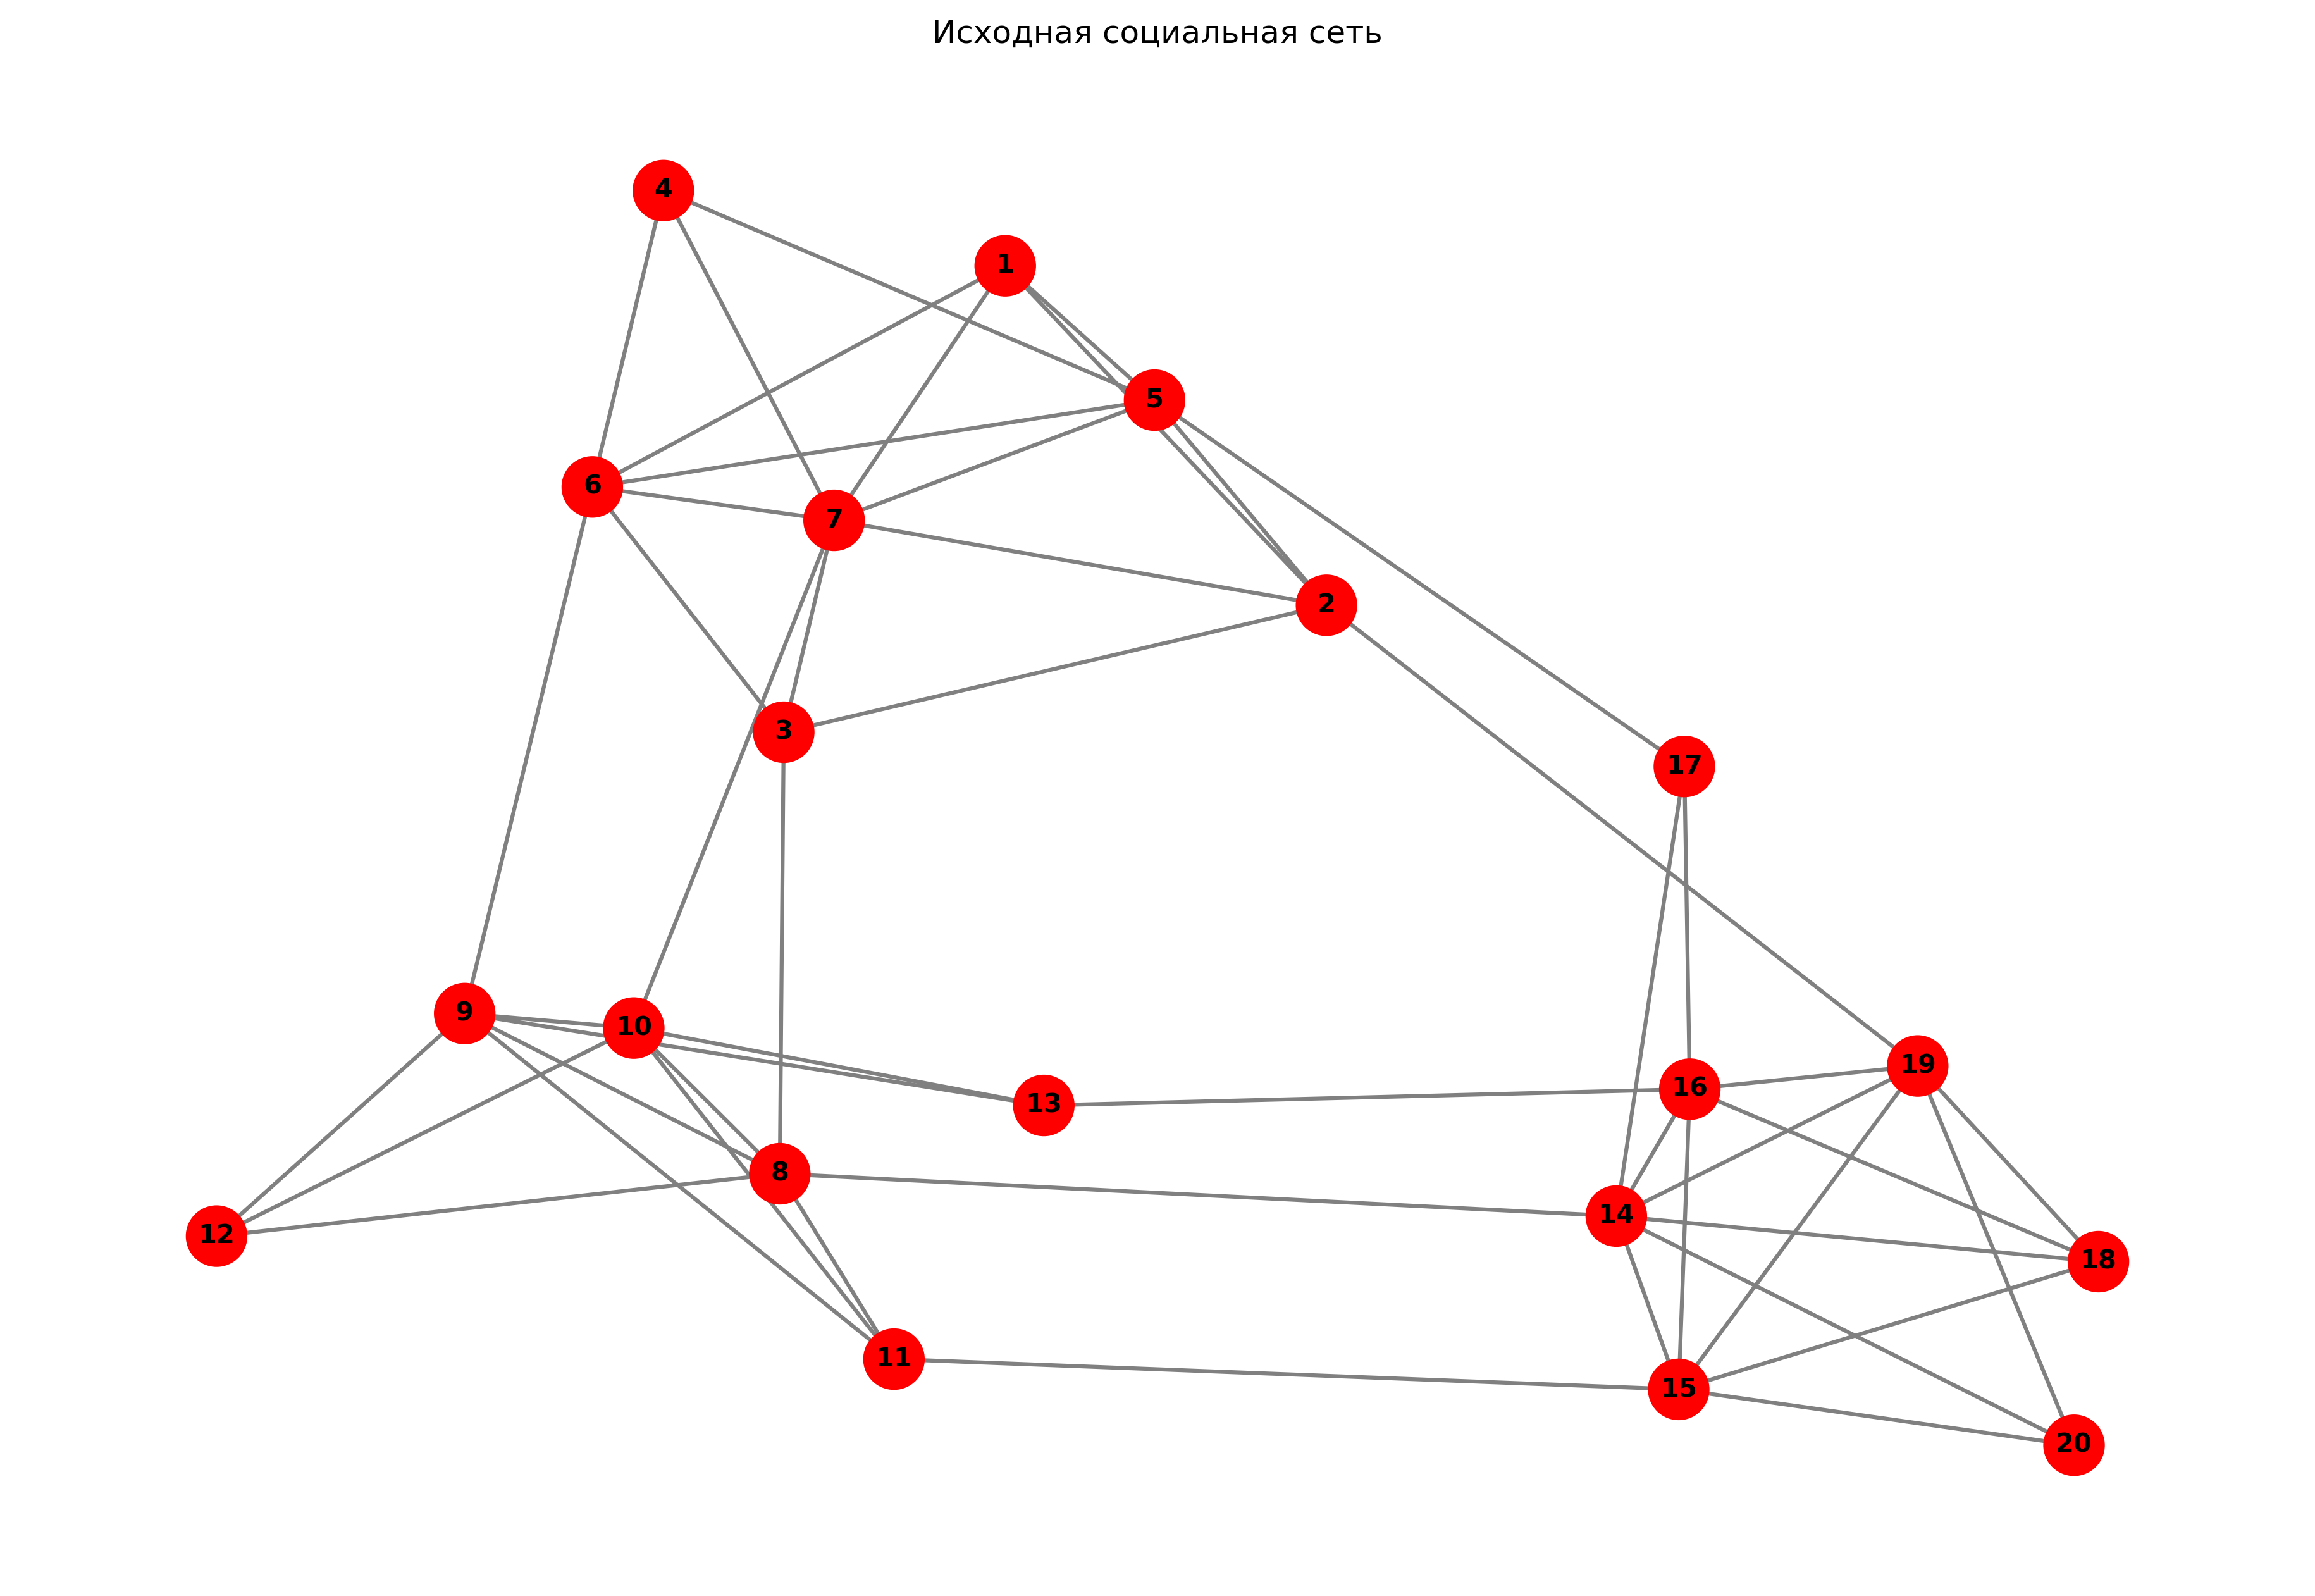
\includegraphics[width=0.9\textwidth]{images/task1/original_network.png}
    \caption{Исходная социальная сеть}
\end{figure}

\subsection*{Анализ собственных чисел матрицы Лапласа}

\begin{figure}[H]
    \centering
    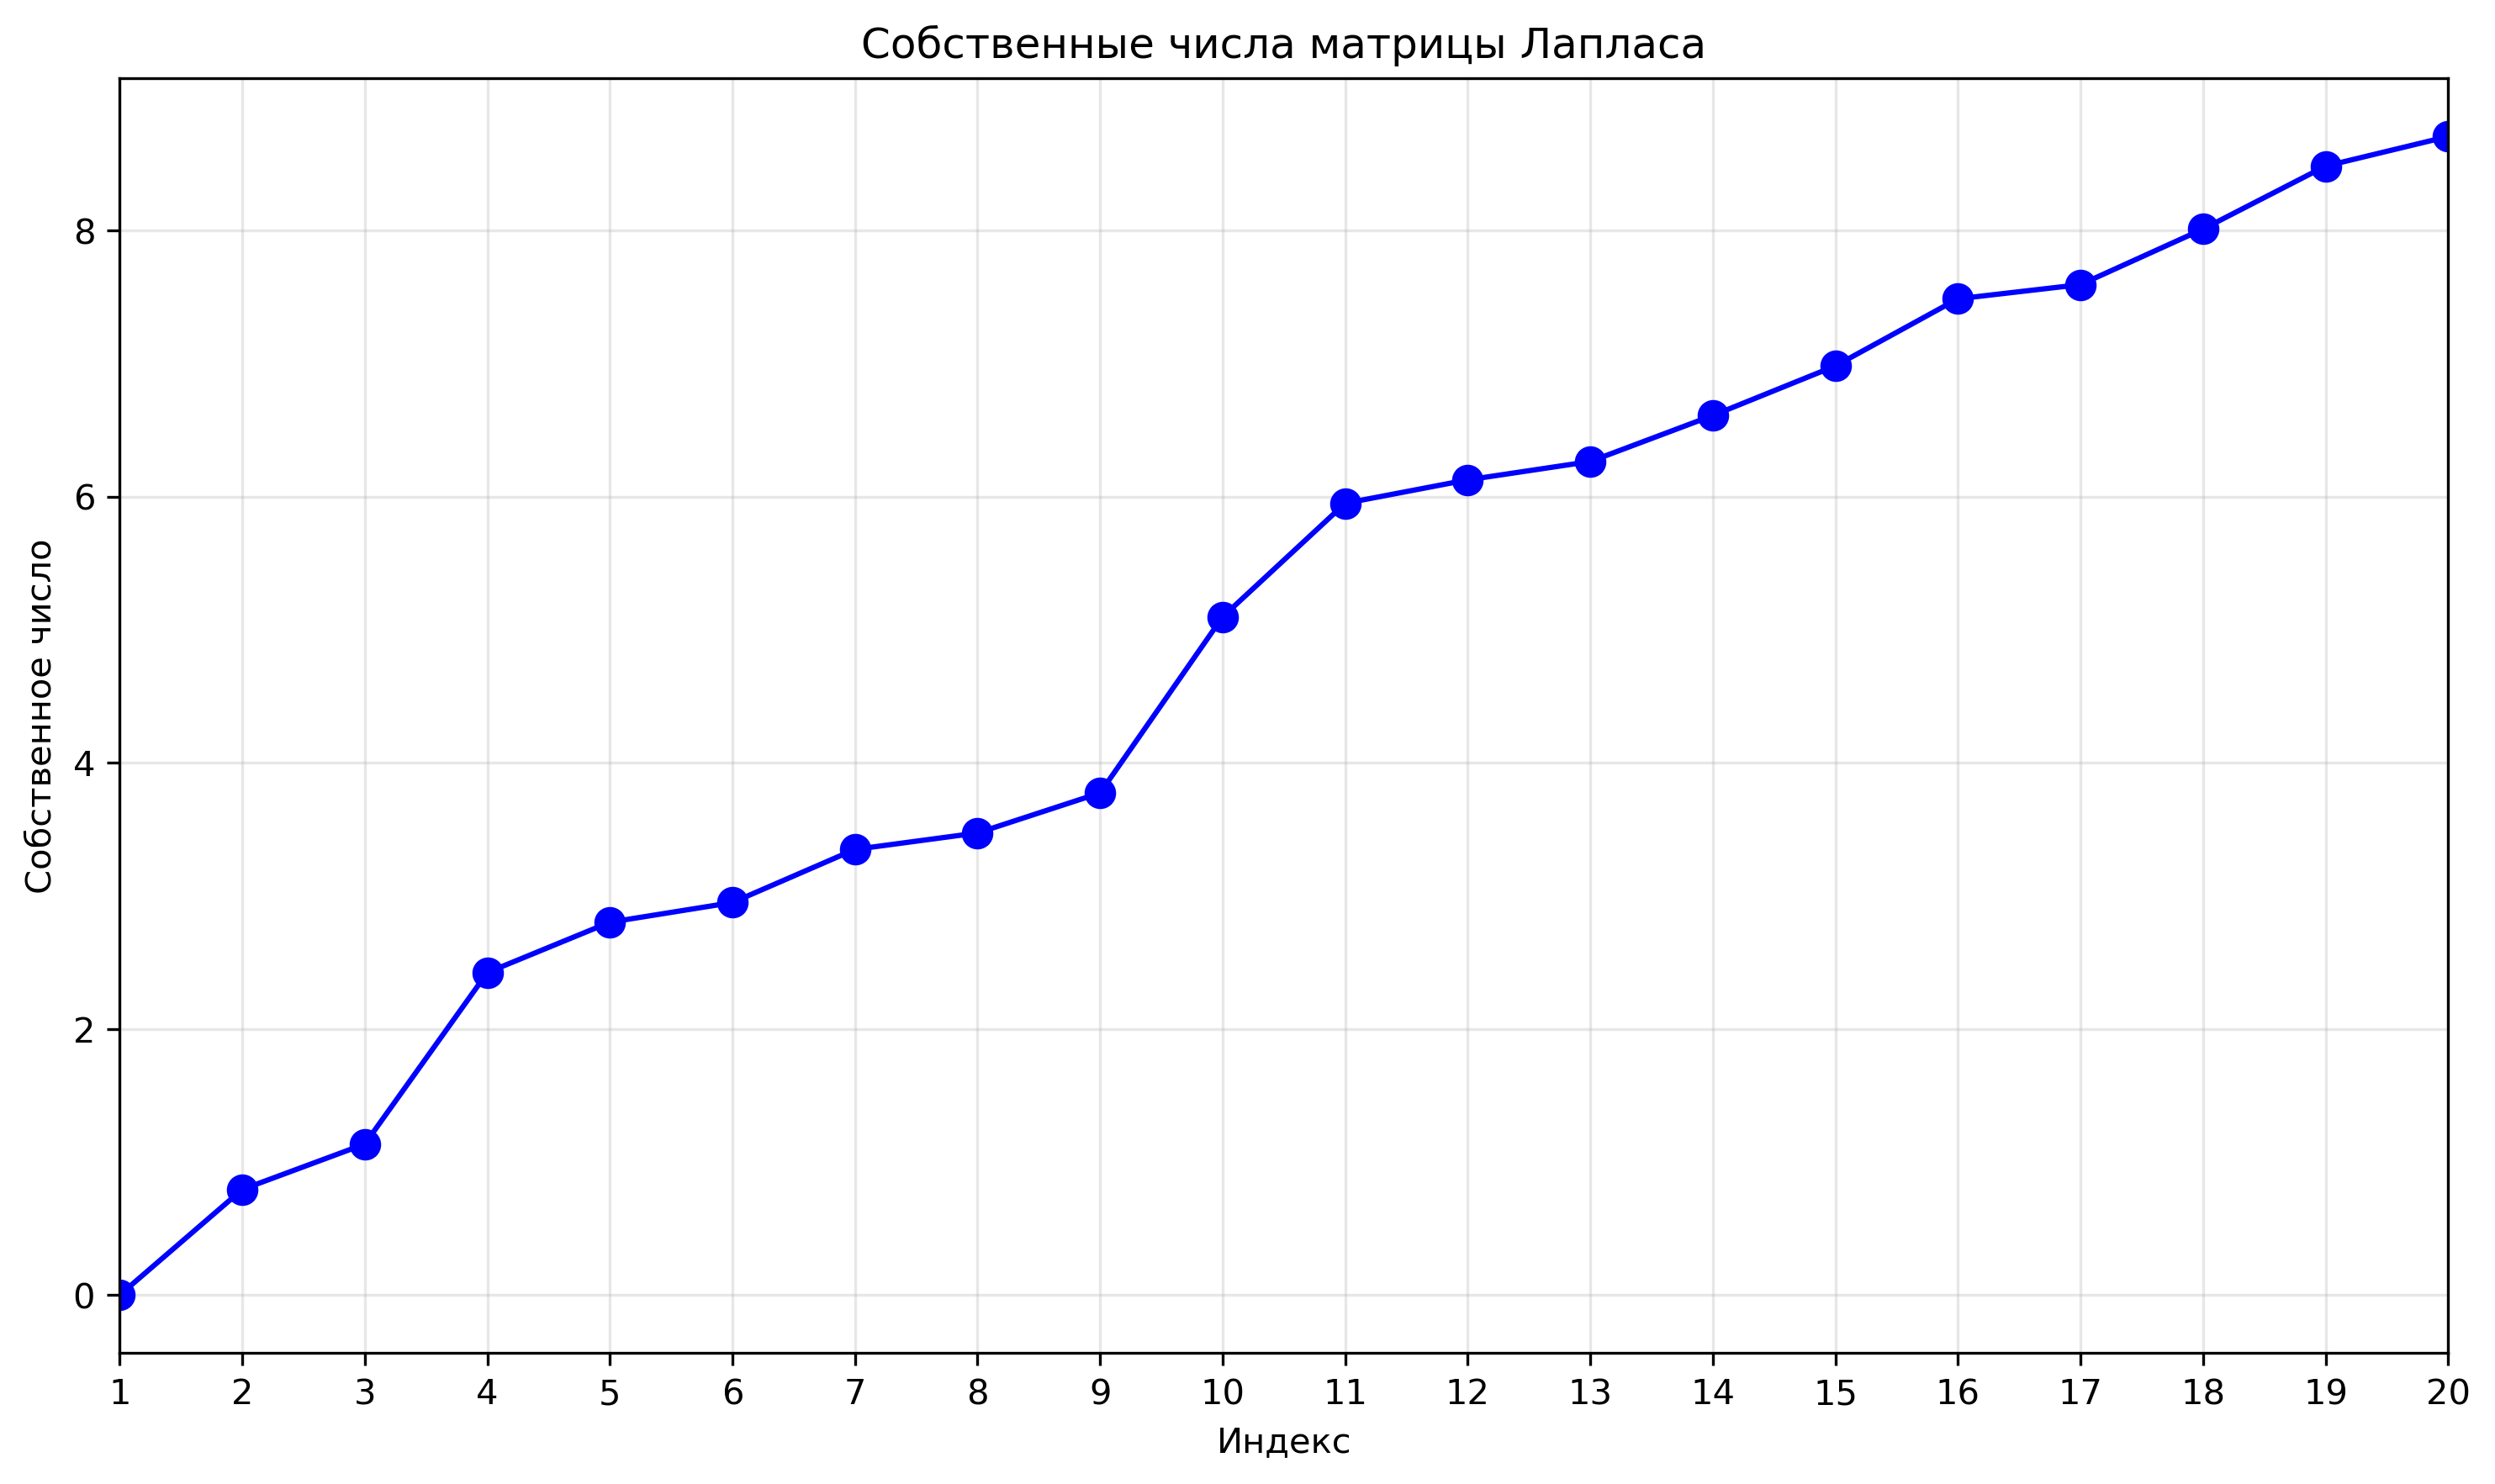
\includegraphics[width=0.9\textwidth]{images/task1/eigenvalues.png}
    \caption{Собственные числа матрицы Лапласа}
\end{figure}

Наблюдаемые собственные числа:
\begin{itemize}
    \item $\lambda_1 = 0.0000$ (наименьшее, соответствует связности графа)
    \item $\lambda_2 = 0.7154$ (первое ненулевое)
    \item $\lambda_3 = 1.0539$
    \item $\lambda_4 = 1.6731$
    \item $\lambda_5 = 1.8286$
\end{itemize}

\subsection*{Методика расчёта Silhouette score}

Для оценки качества кластеризации использовался показатель Silhouette score. Для каждой точки $x_i$ он вычисляется как
\[
 s(i) = \frac{b(i) - a(i)}{\max\{a(i), \, b(i)\}},
\]
где $a(i)$ — среднее внутрикластерное расстояние от точки $i$ до остальных точек её кластера, а $b(i)$ — минимальное среднее межкластерное расстояние от точки $i$ до точек ближайшего другого кластера. Итоговый Silhouette score — это среднее значение $s(i)$ по всем точкам; он лежит в диапазоне от $-1$ до $1$ (чем больше, тем лучше разделены кластеры).

В рамках спектральной кластеризации точки для оценки — это строки матрицы $V = [v_1,\ldots,v_k]$, где $v_j$ — собственные векторы матрицы Лапласа, соответствующие $k$ наименьшим собственным числам (без нулевого). Таким образом, каждая вершина графа представляется вектором признаков из $\mathbb{R}^k$ — соответствующей строкой матрицы $V$.

Практически вычисление выполнялось с помощью функции \texttt{silhouette\_score} из пакета \texttt{scikit-learn} c евклидовой метрикой по умолчанию. В коде это соответствует вызову:
\begin{lstlisting}
from sklearn.metrics import silhouette_score
silhouette_avg = silhouette_score(V, clusters)
\end{lstlisting}
где \texttt{V} — матрица размеров $n\times k$ (строки — точки в $\mathbb{R}^k$), а \texttt{clusters} — метки кластеров, полученные методом \texttt{KMeans}.

\subsection*{Результаты кластеризации для различных k}

\subsubsection*{k = 2}

\begin{figure}[H]
    \centering
    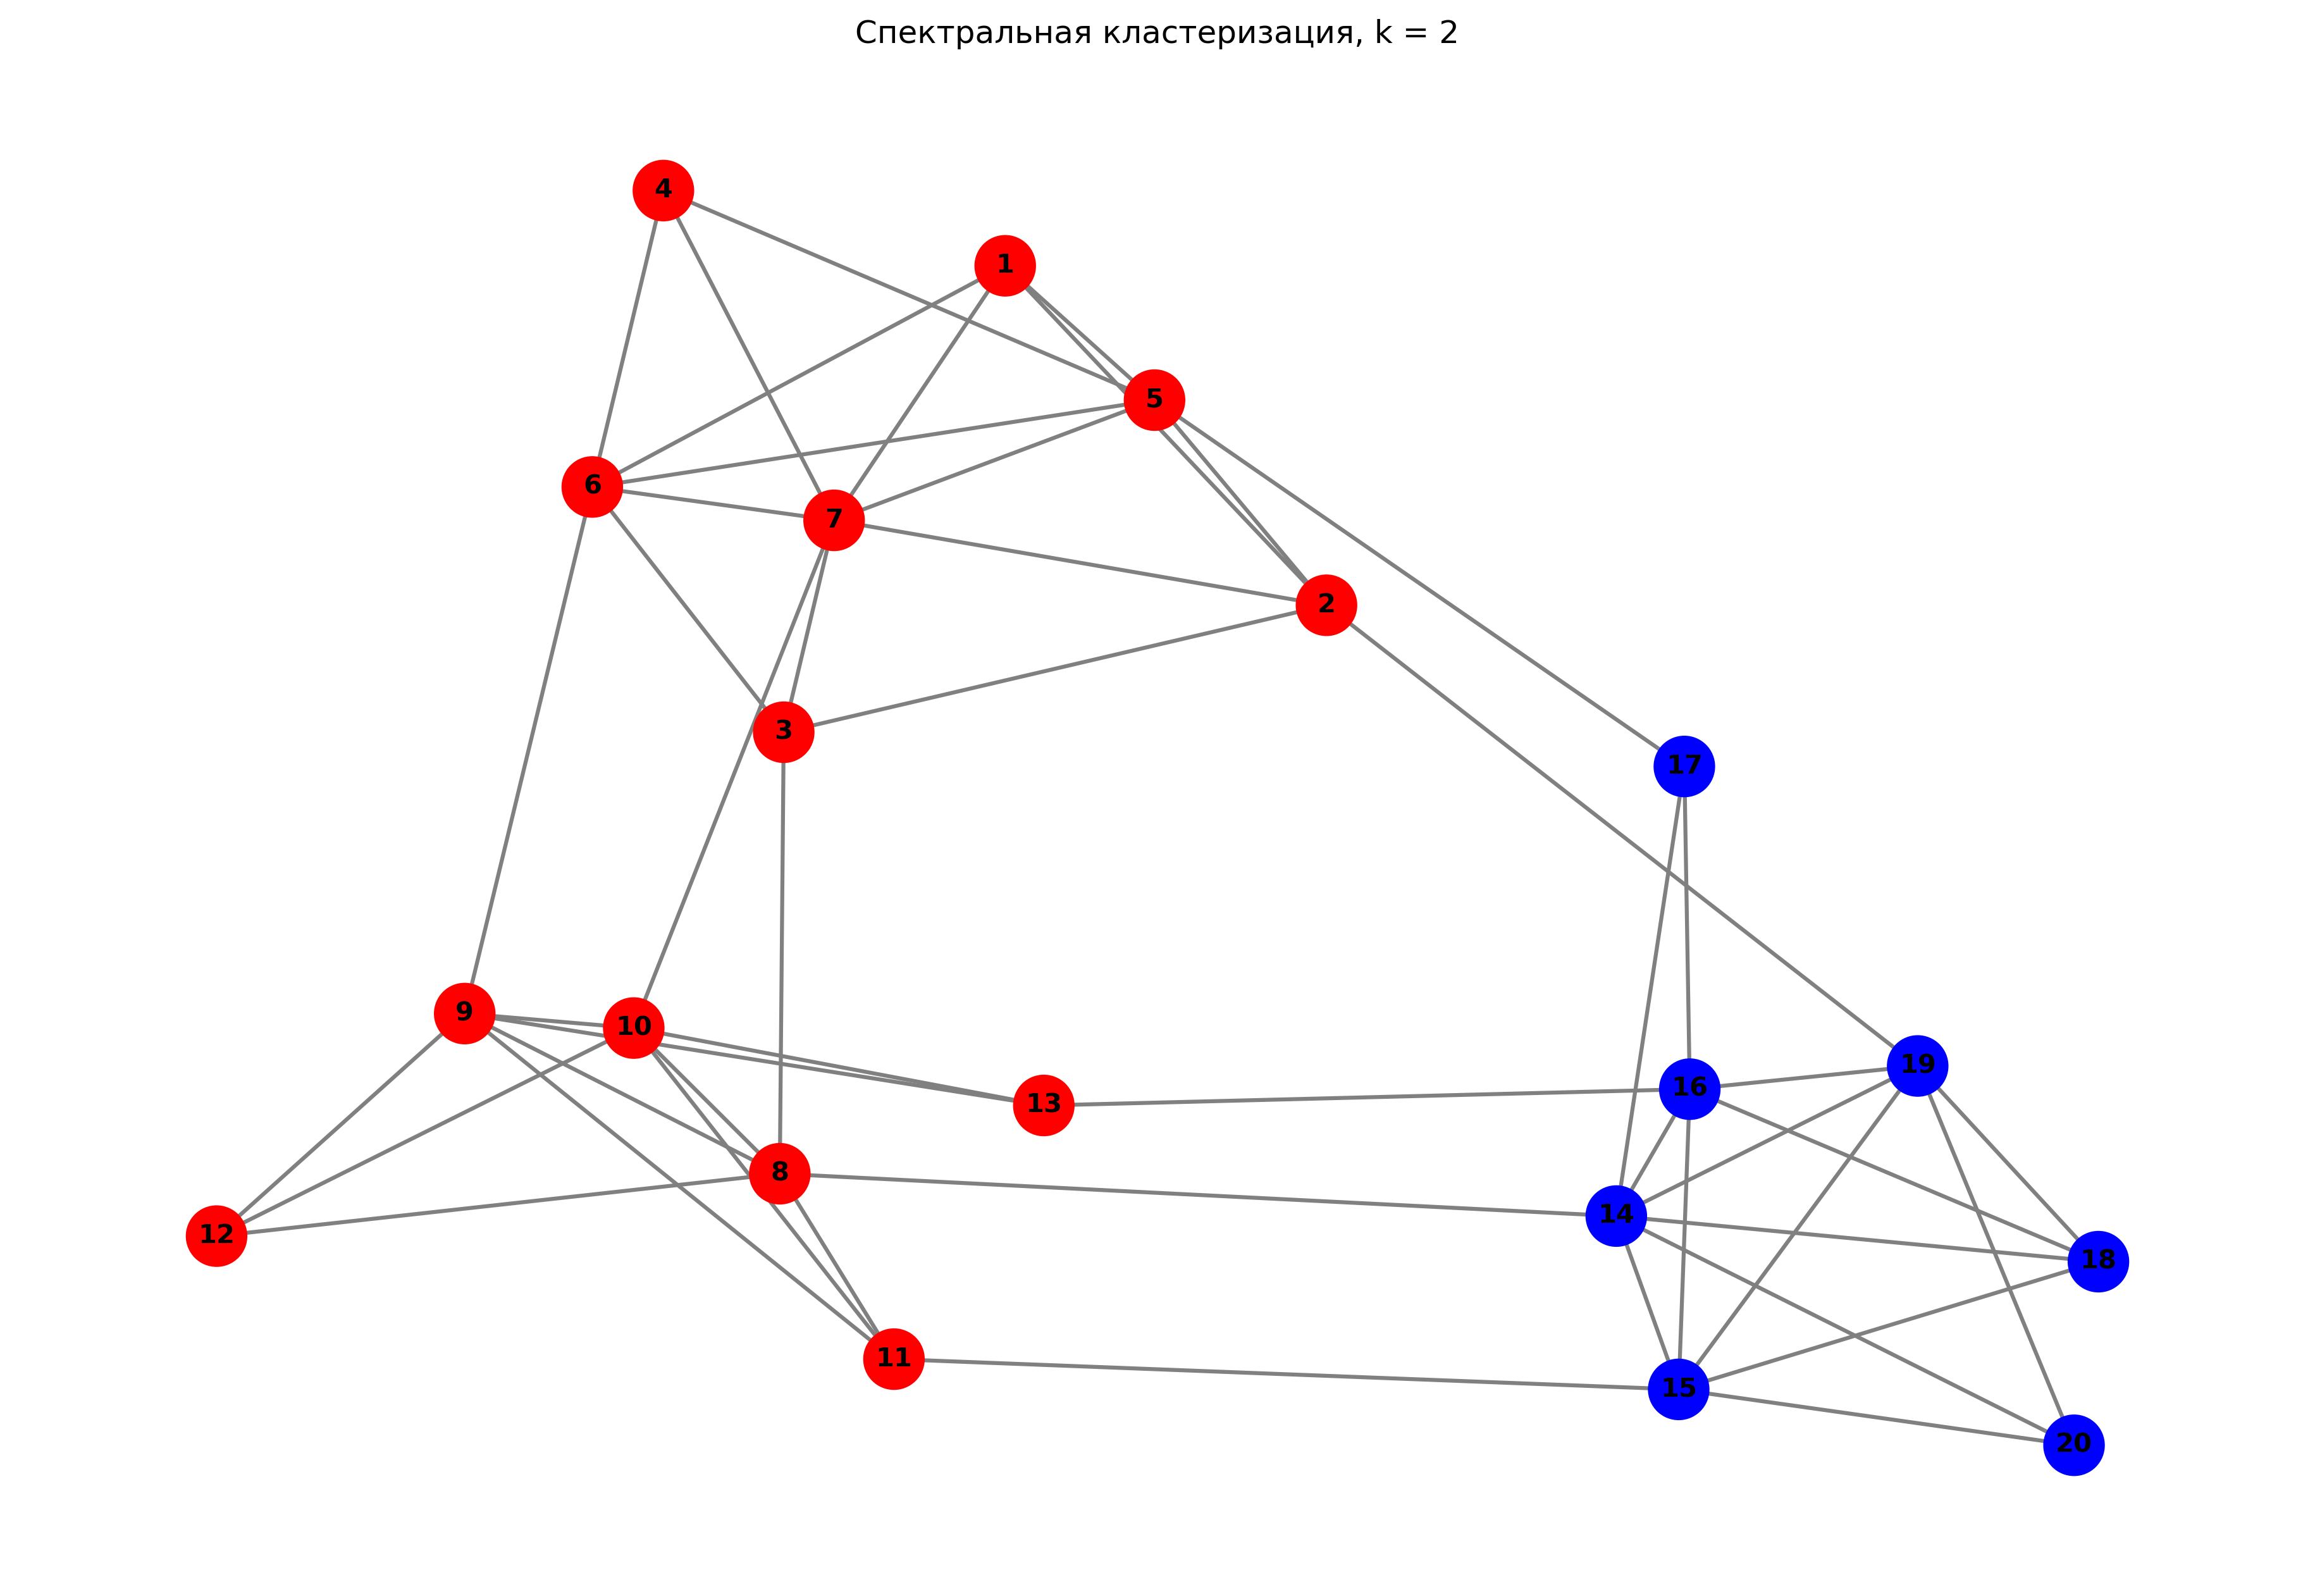
\includegraphics[width=0.9\textwidth]{images/task1/clustering_k2.png}
    \caption{Спектральная кластеризация, k = 2}
\end{figure}

\textbf{Результаты:}
\begin{itemize}
    \item Silhouette score: 0.4532
    \item Доля внутренних связей: 88.10\%
    \item Внутренние связи: 37, внешние связи: 5
\end{itemize}

\subsubsection*{k = 3}

\begin{figure}[H]
    \centering
    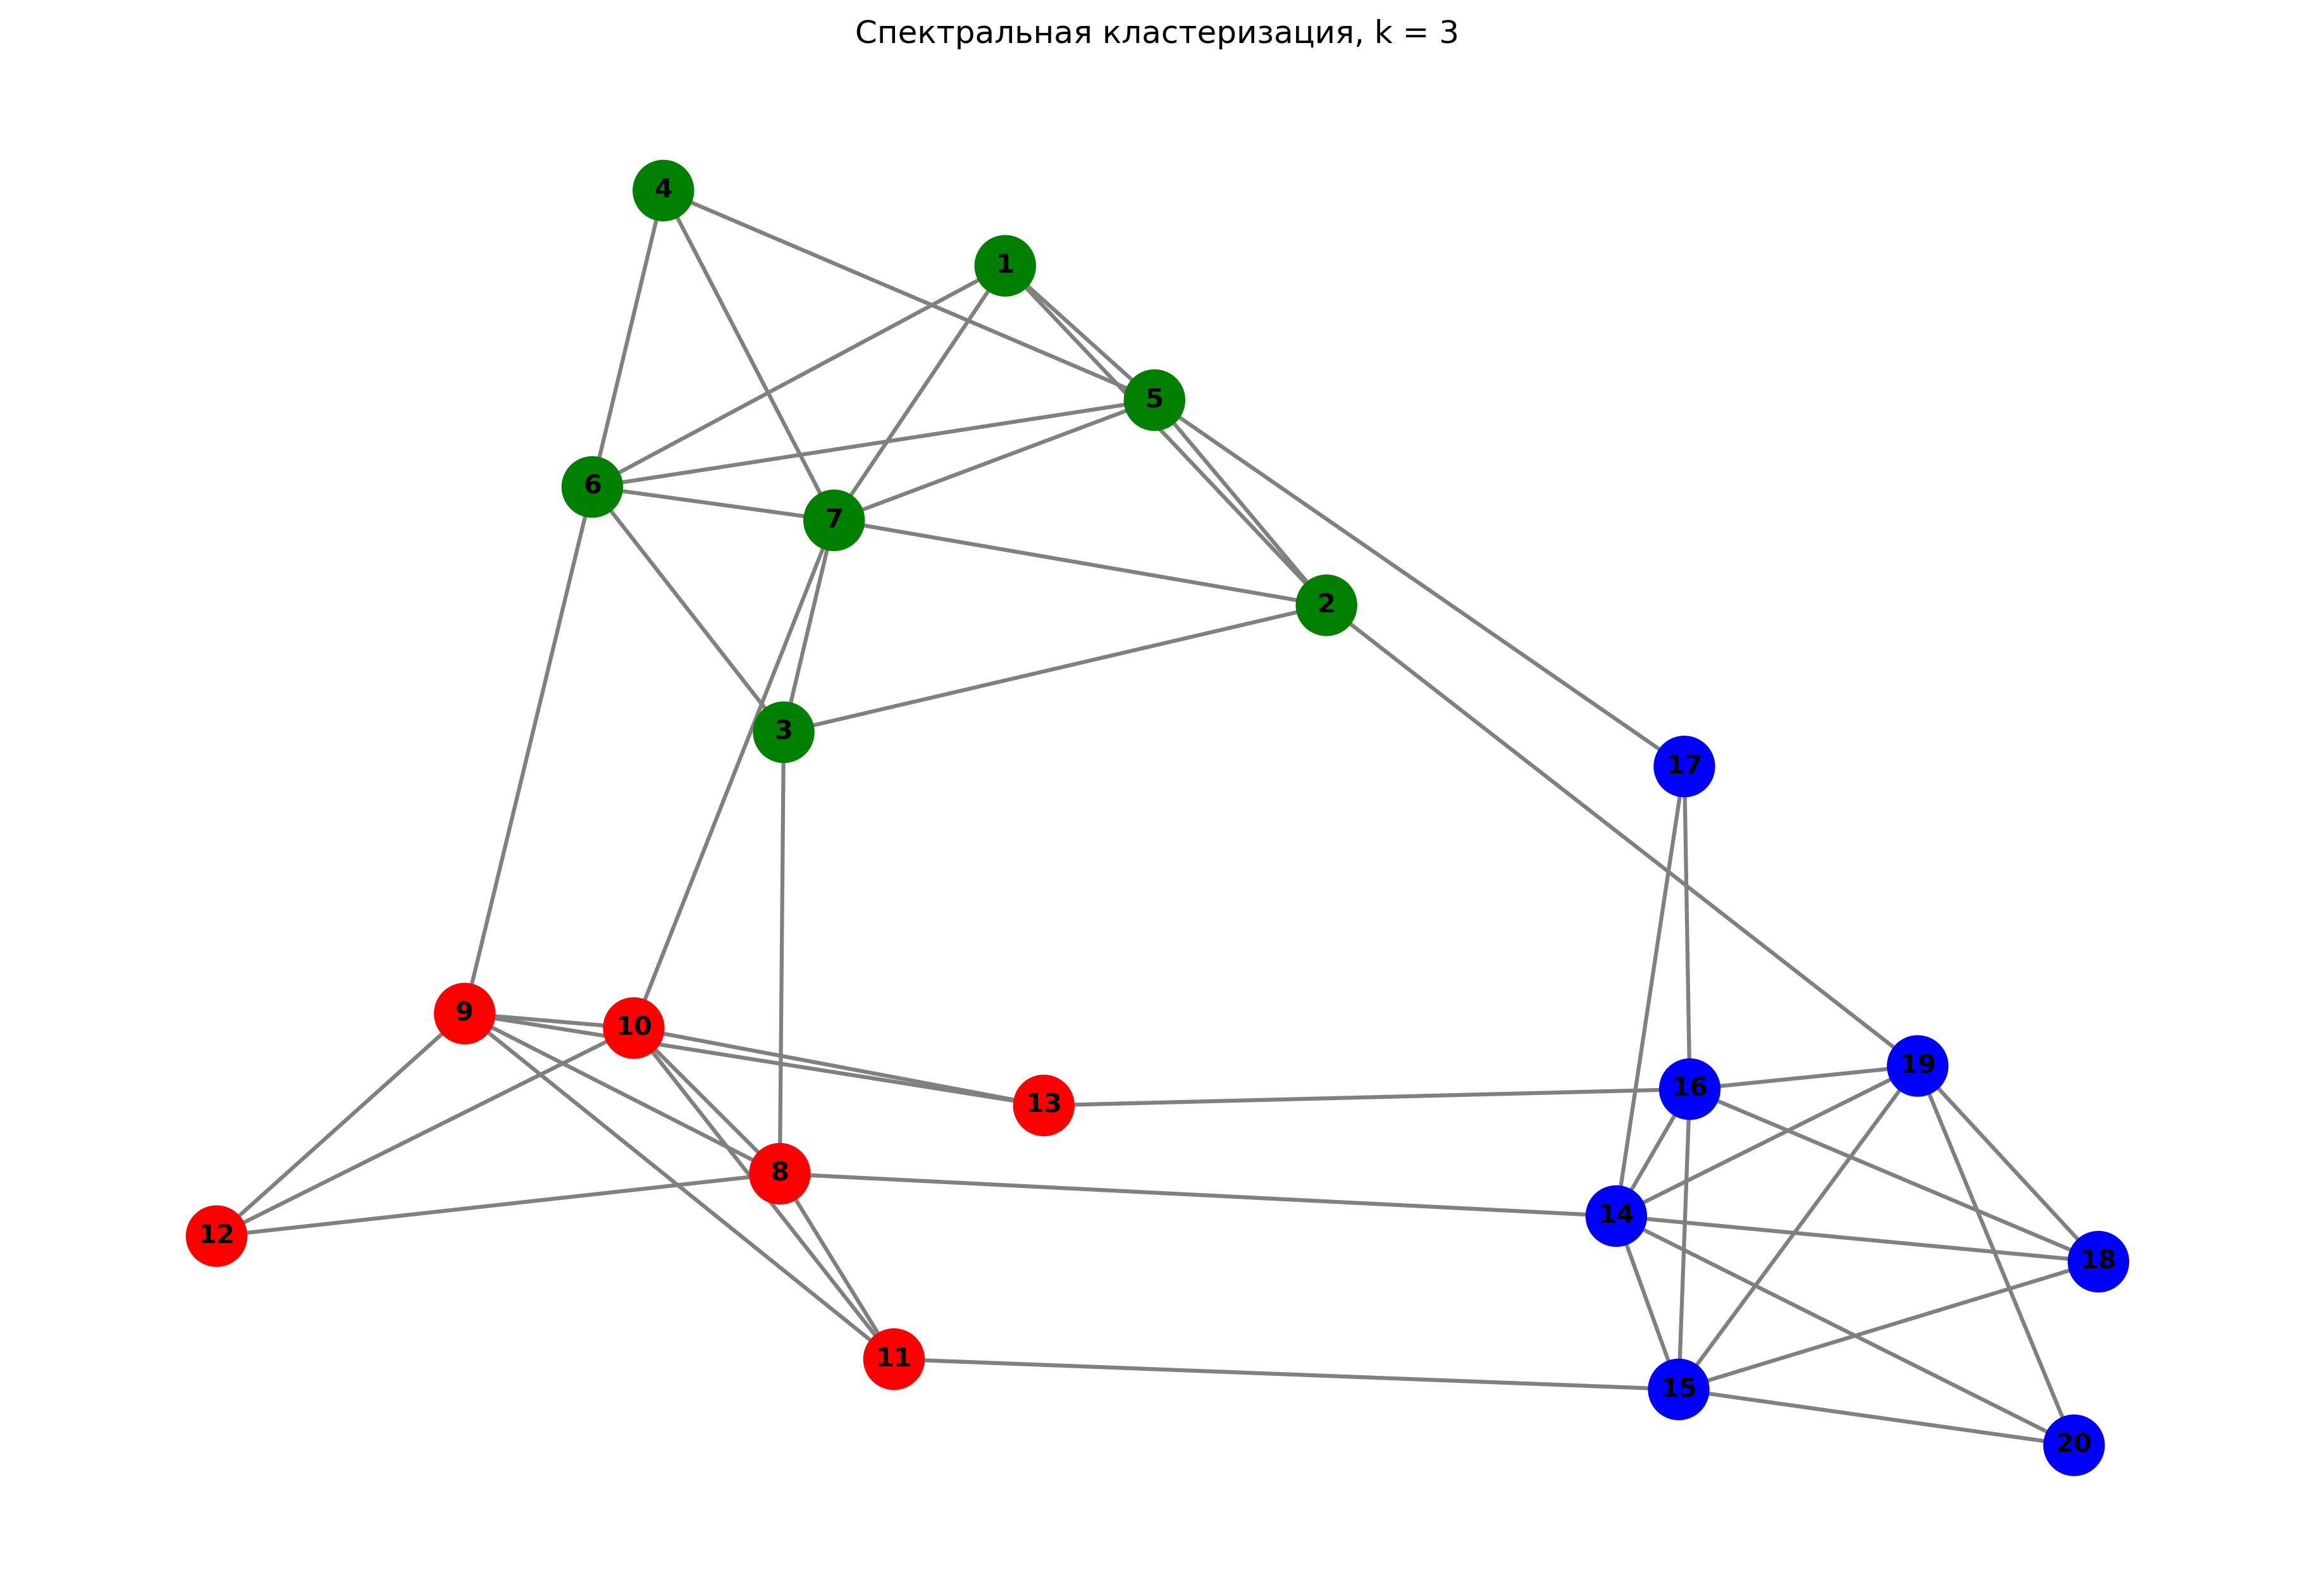
\includegraphics[width=0.9\textwidth]{images/task1/clustering_k3.png}
    \caption{Спектральная кластеризация, k = 3}
\end{figure}

\textbf{Результаты:}
\begin{itemize}
    \item Silhouette score: 0.4580
    \item Доля внутренних связей: 80.95\%
    \item Внутренние связи: 34, внешние связи: 8
\end{itemize}

\subsubsection*{k = 4}

\begin{figure}[H]
    \centering
    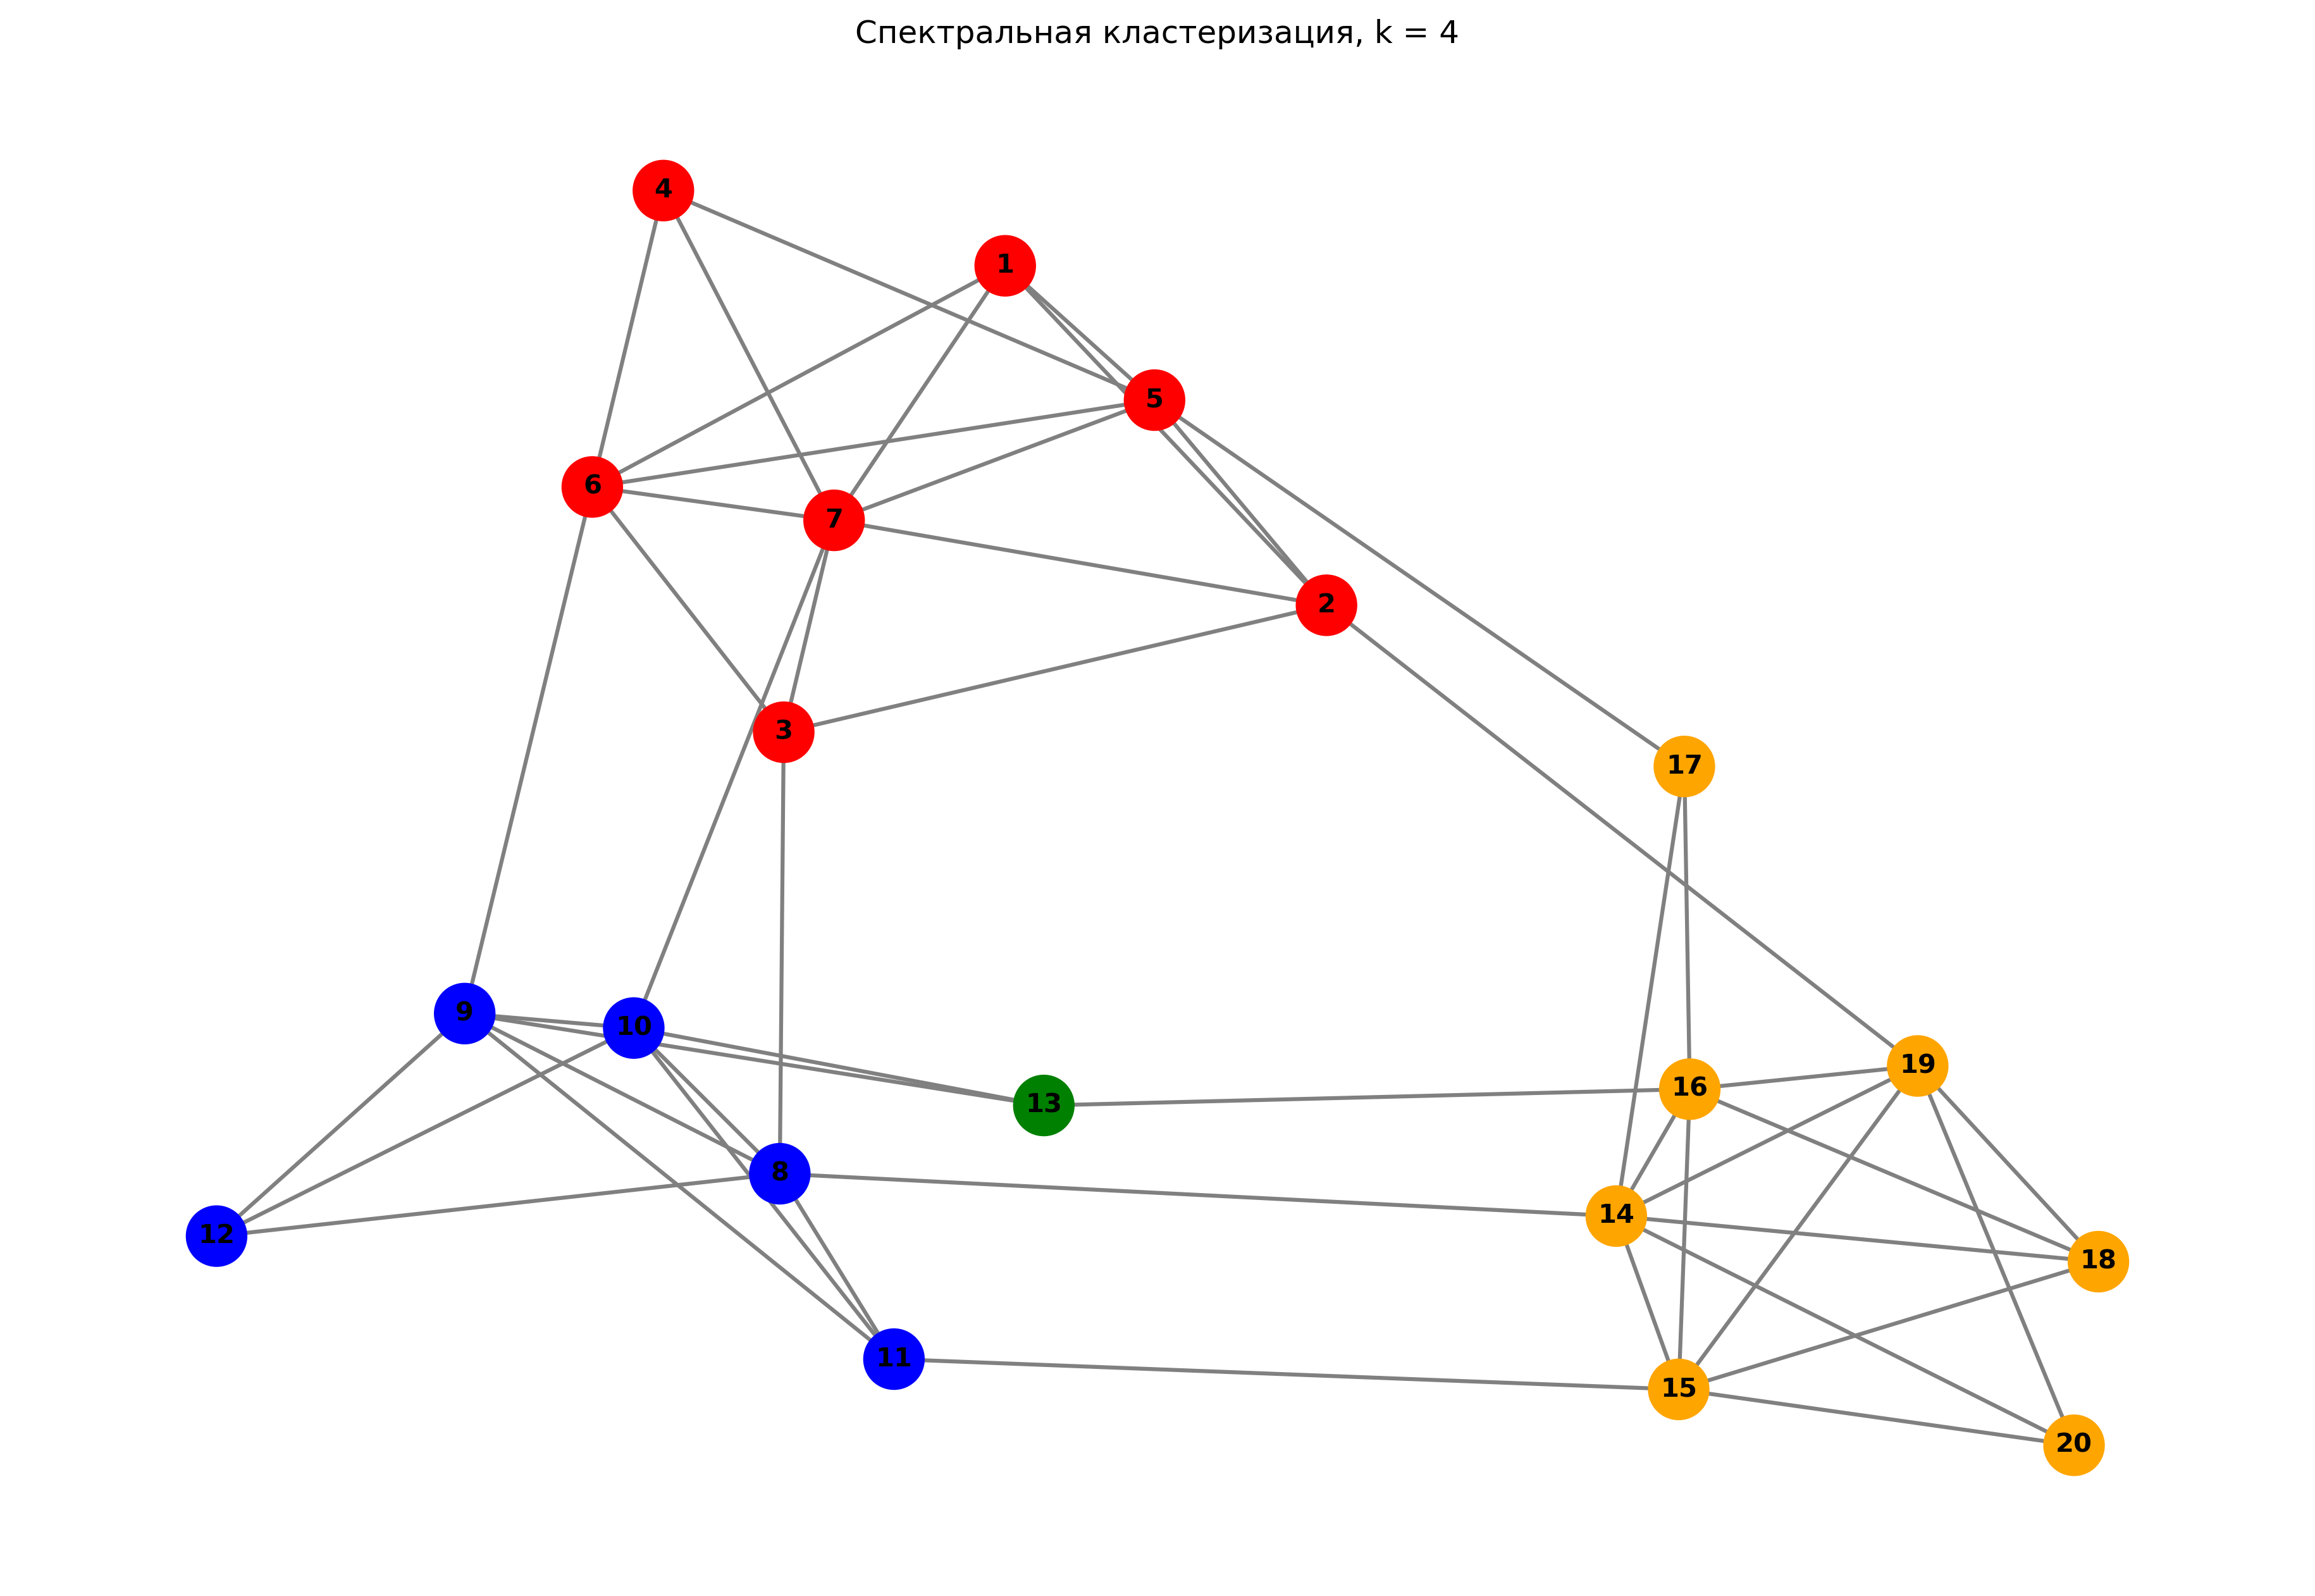
\includegraphics[width=0.9\textwidth]{images/task1/clustering_k4.png}
    \caption{Спектральная кластеризация, k = 4}
\end{figure}

\textbf{Результаты:}
\begin{itemize}
    \item Silhouette score: 0.4615 (наилучший)
    \item Доля внутренних связей: 71.43\%
    \item Внутренние связи: 30, внешние связи: 12
\end{itemize}

\subsubsection*{k = 5}

\begin{figure}[H]
    \centering
    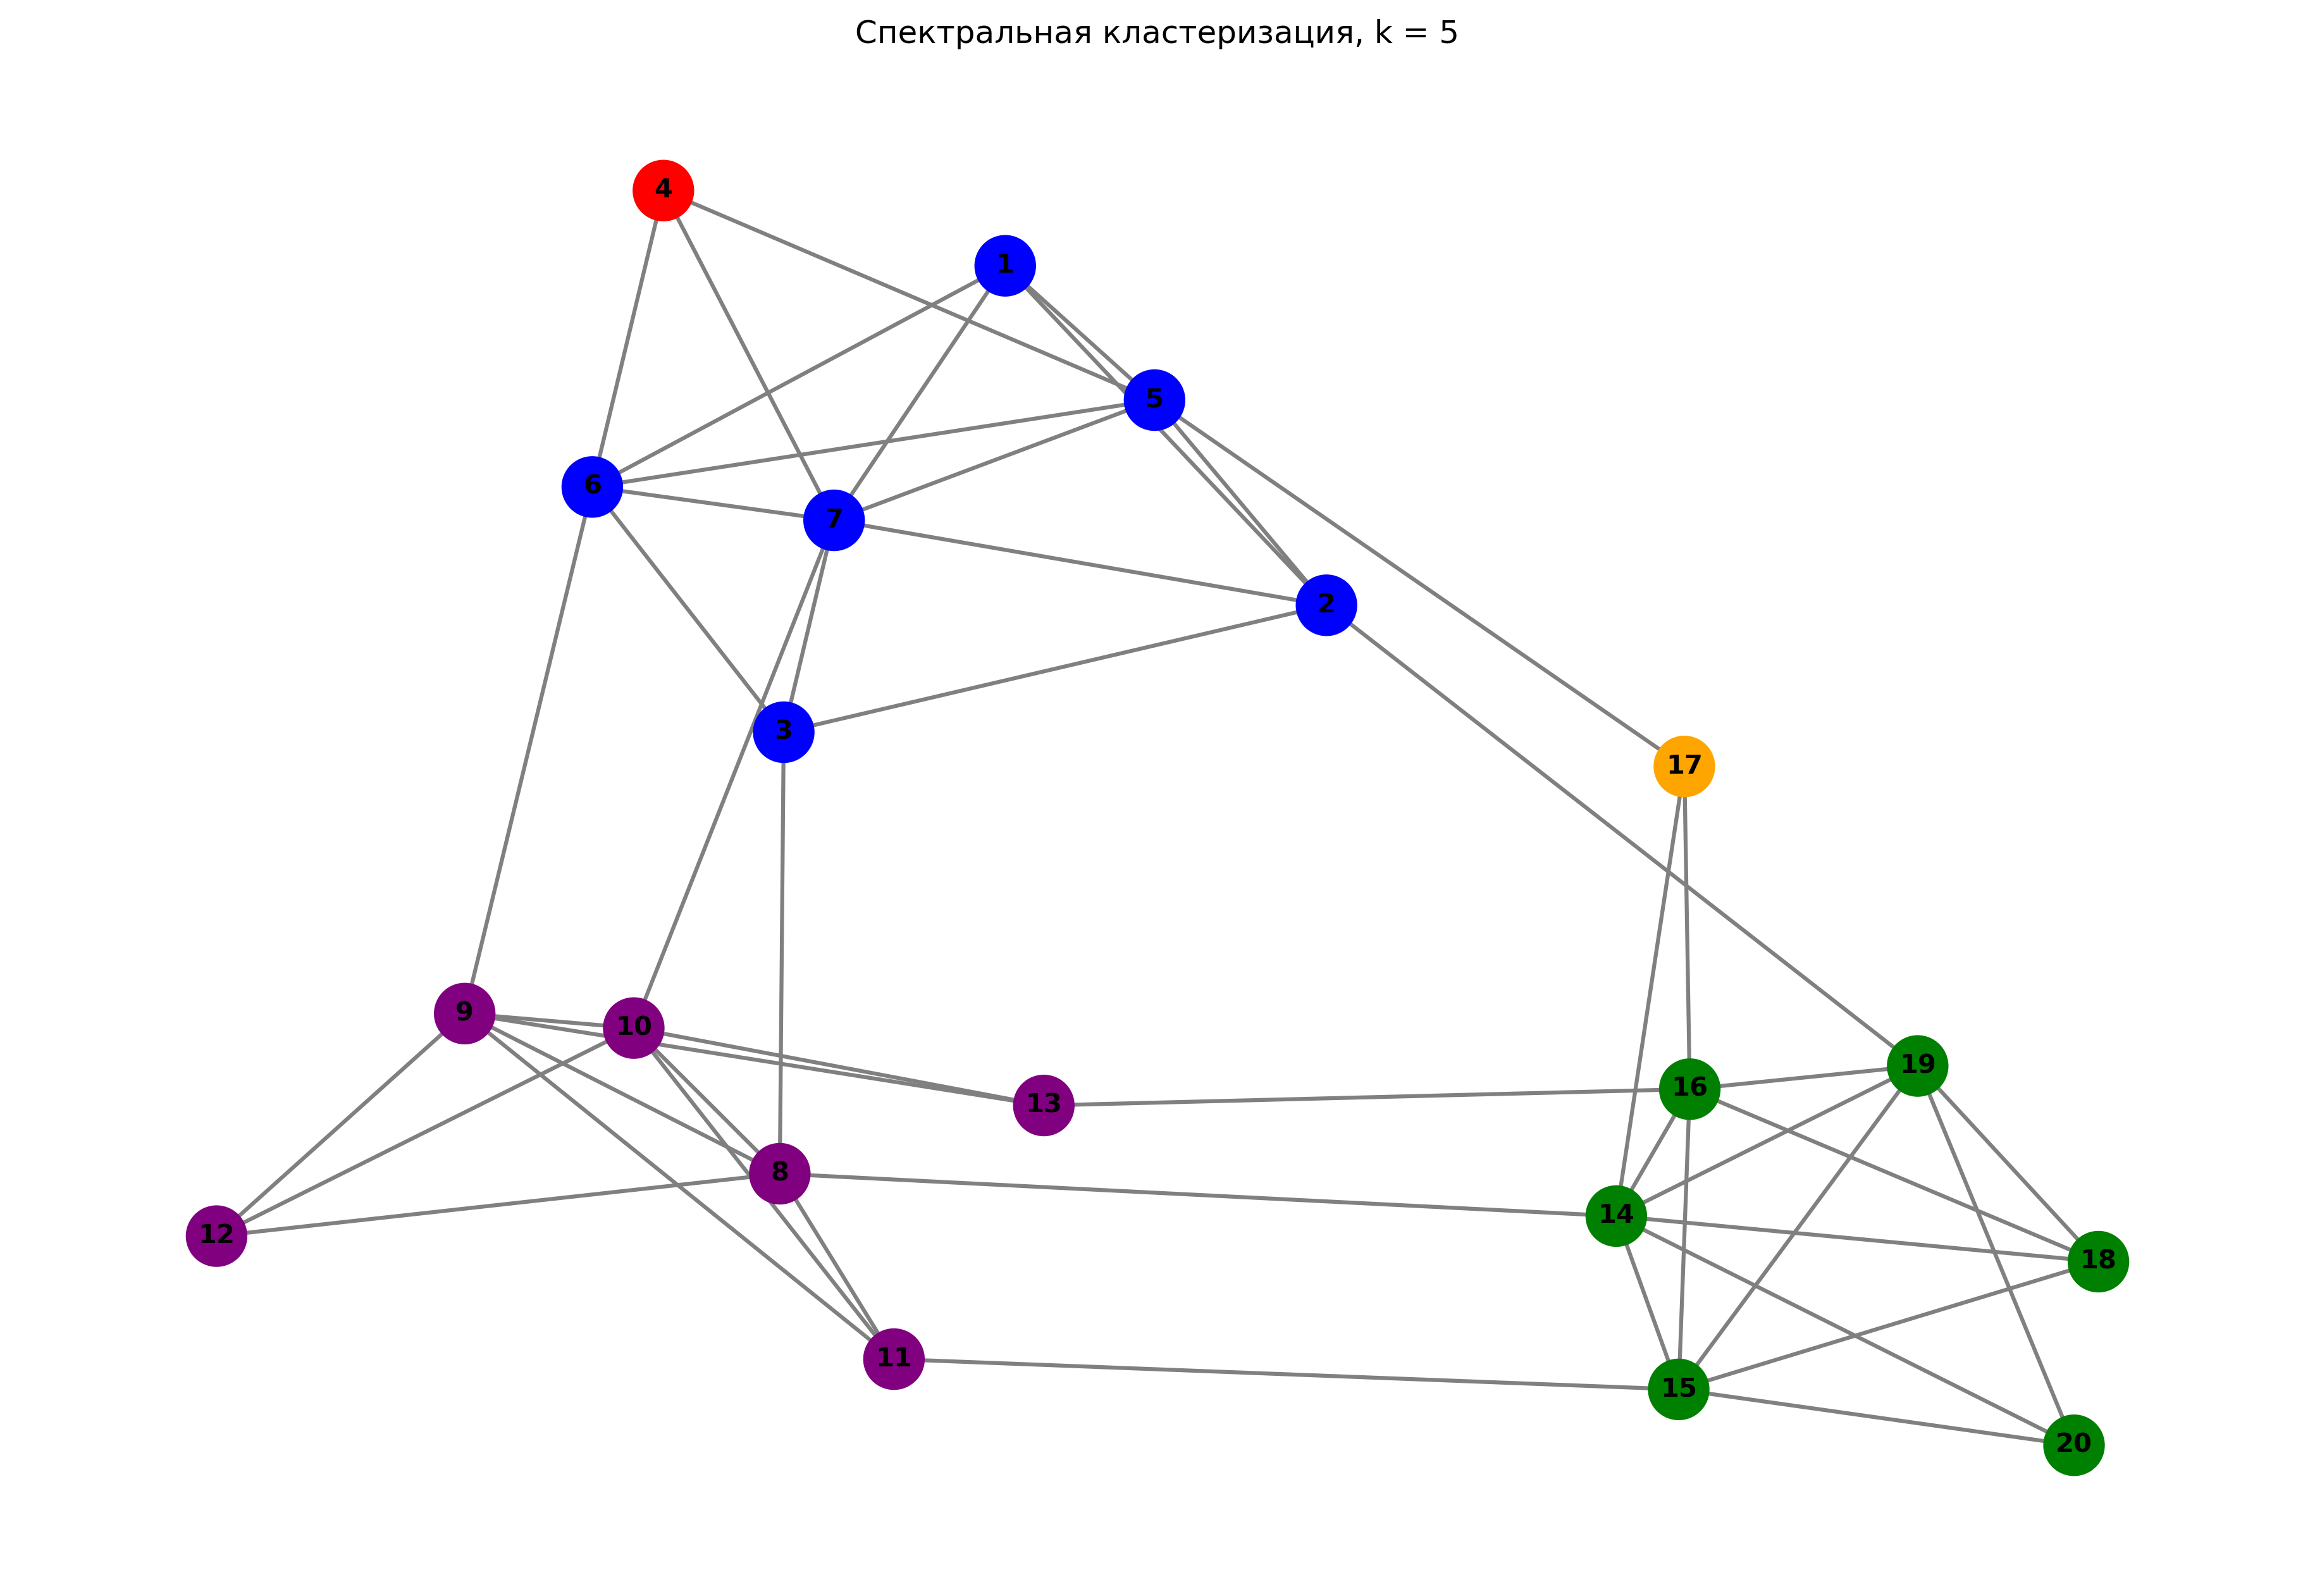
\includegraphics[width=0.9\textwidth]{images/task1/clustering_k5.png}
    \caption{Спектральная кластеризация, k = 5}
\end{figure}

\textbf{Результаты:}
\begin{itemize}
    \item Silhouette score: 0.3683
    \item Доля внутренних связей: 66.67\%
    \item Внутренние связи: 28, внешние связи: 14
\end{itemize}

\subsubsection*{k = 6}

\begin{figure}[H]
    \centering
    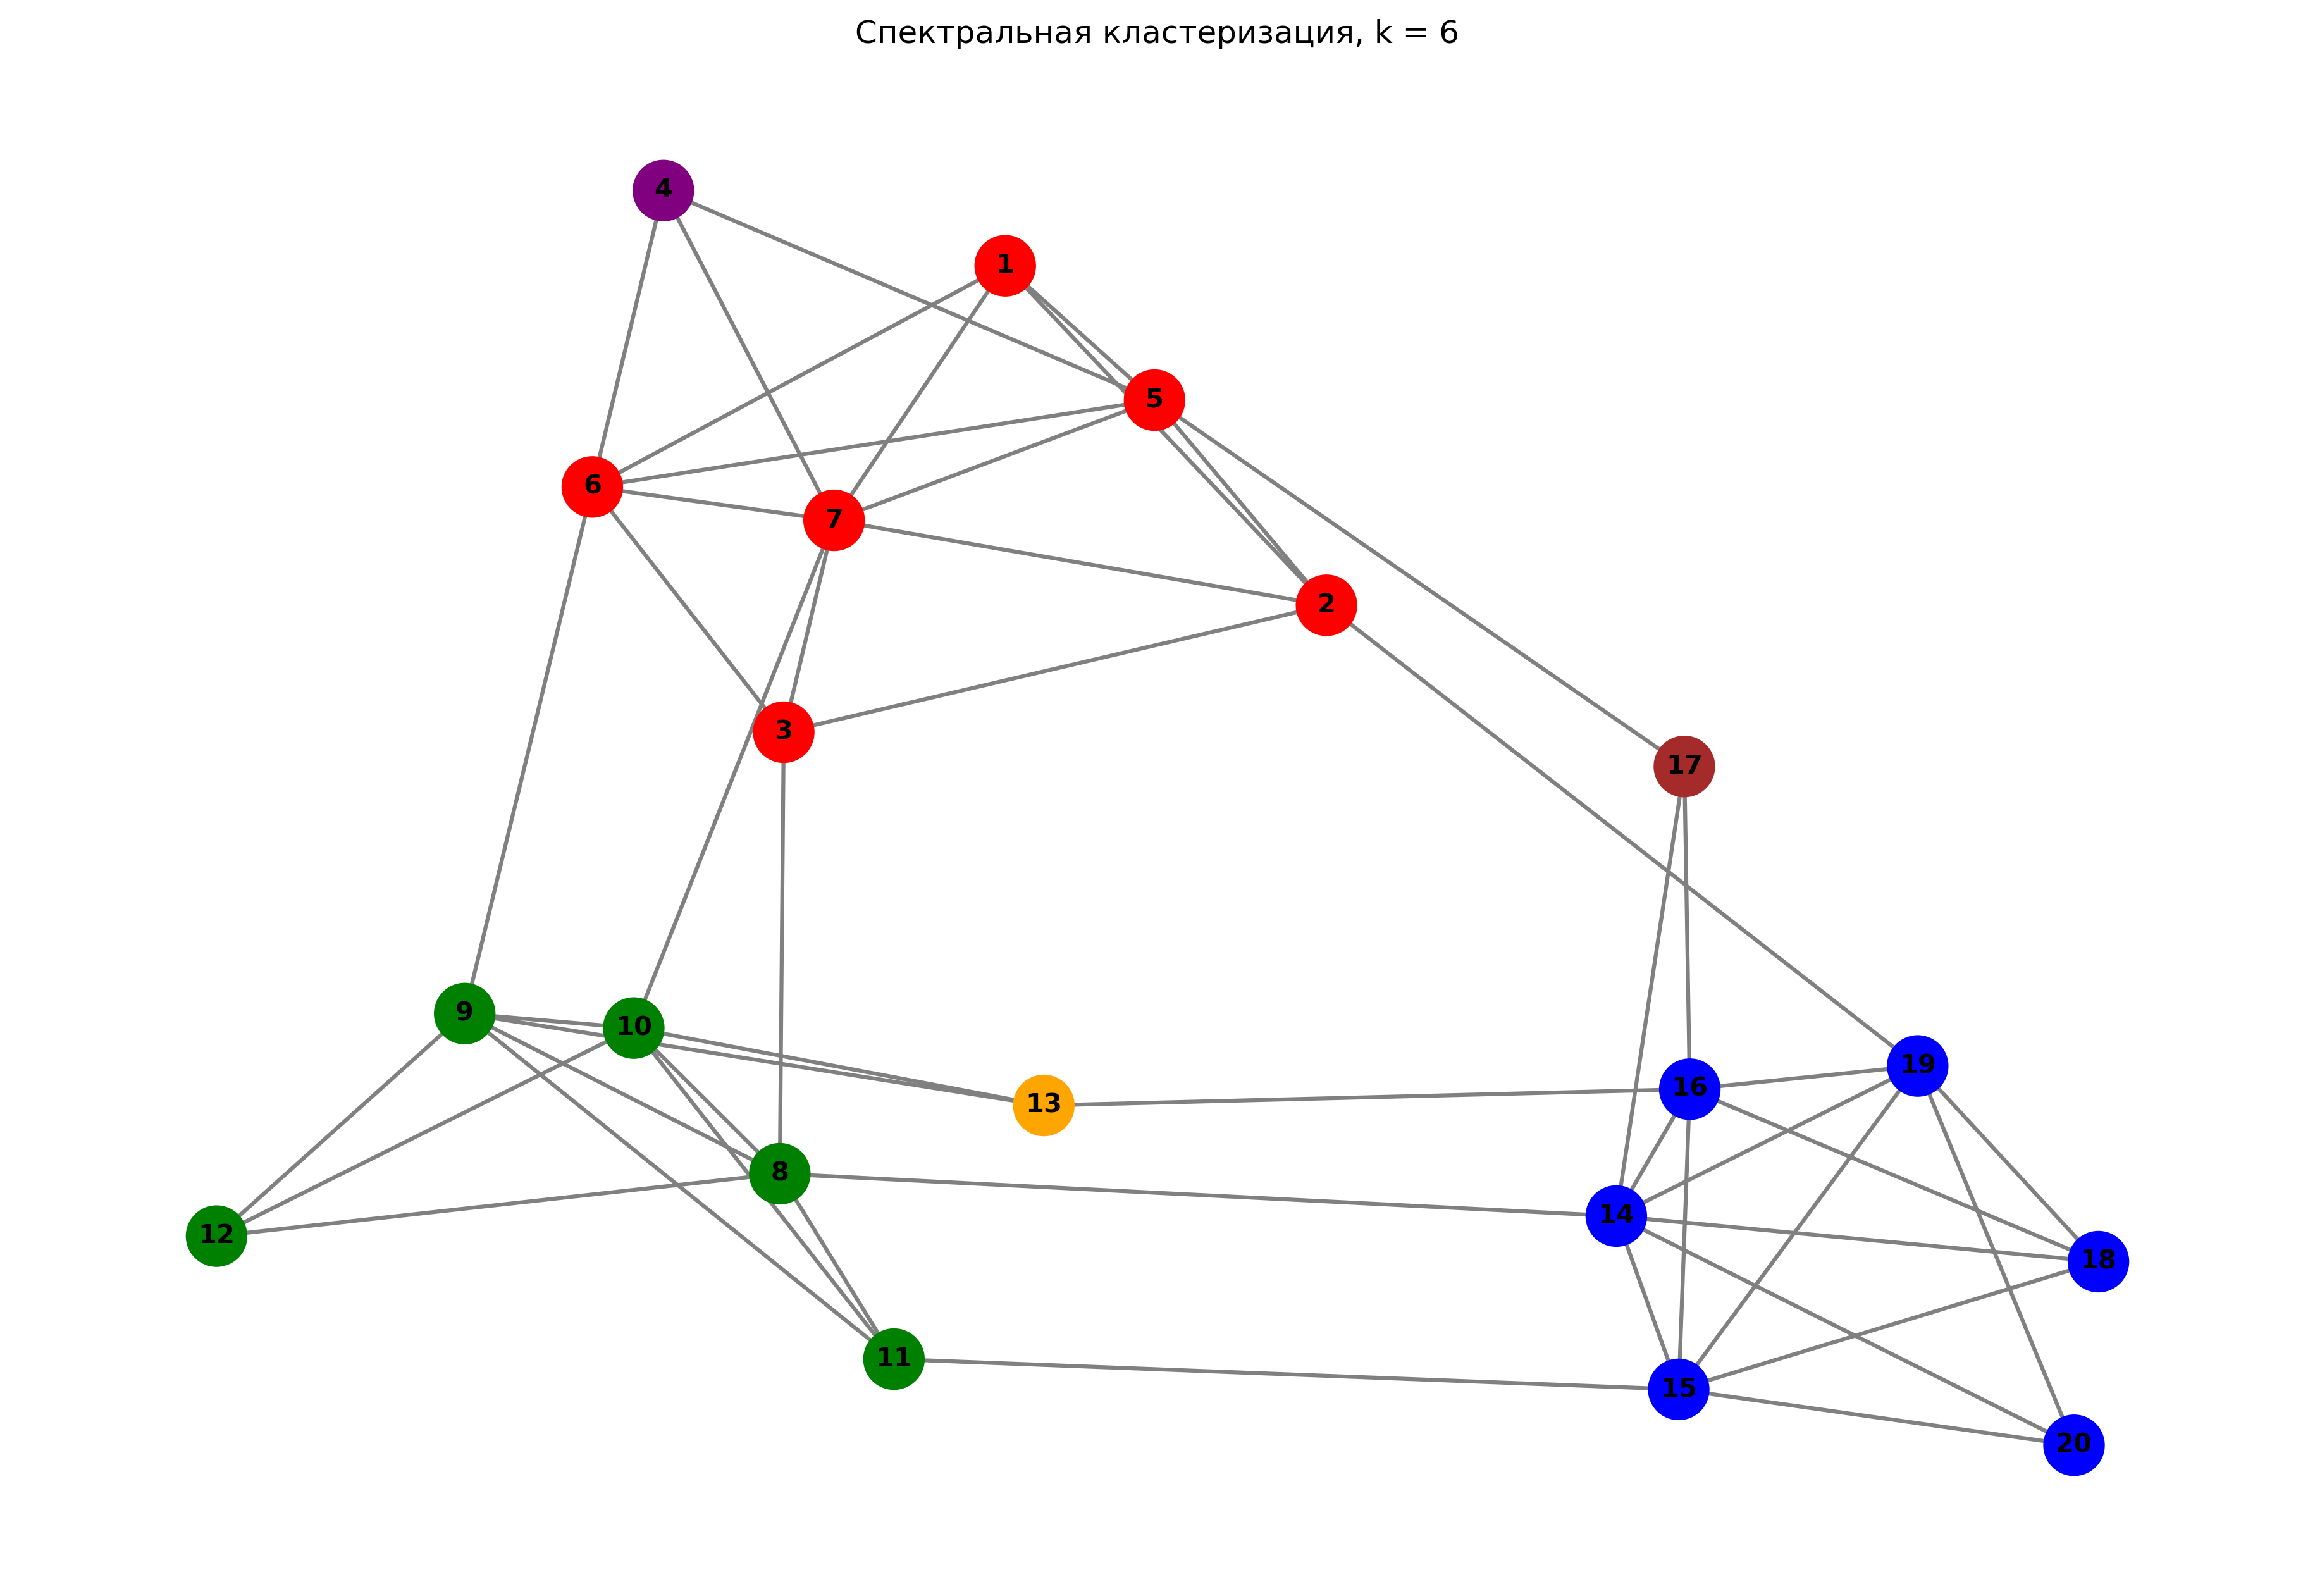
\includegraphics[width=0.9\textwidth]{images/task1/clustering_k6.png}
    \caption{Спектральная кластеризация, k = 6}
\end{figure}

\textbf{Результаты:}
\begin{itemize}
    \item Silhouette score: 0.3546
    \item Доля внутренних связей: 59.52\%
    \item Внутренние связи: 25, внешние связи: 17
\end{itemize}

\subsection*{Сравнительный анализ}

\begin{figure}[H]
    \centering
    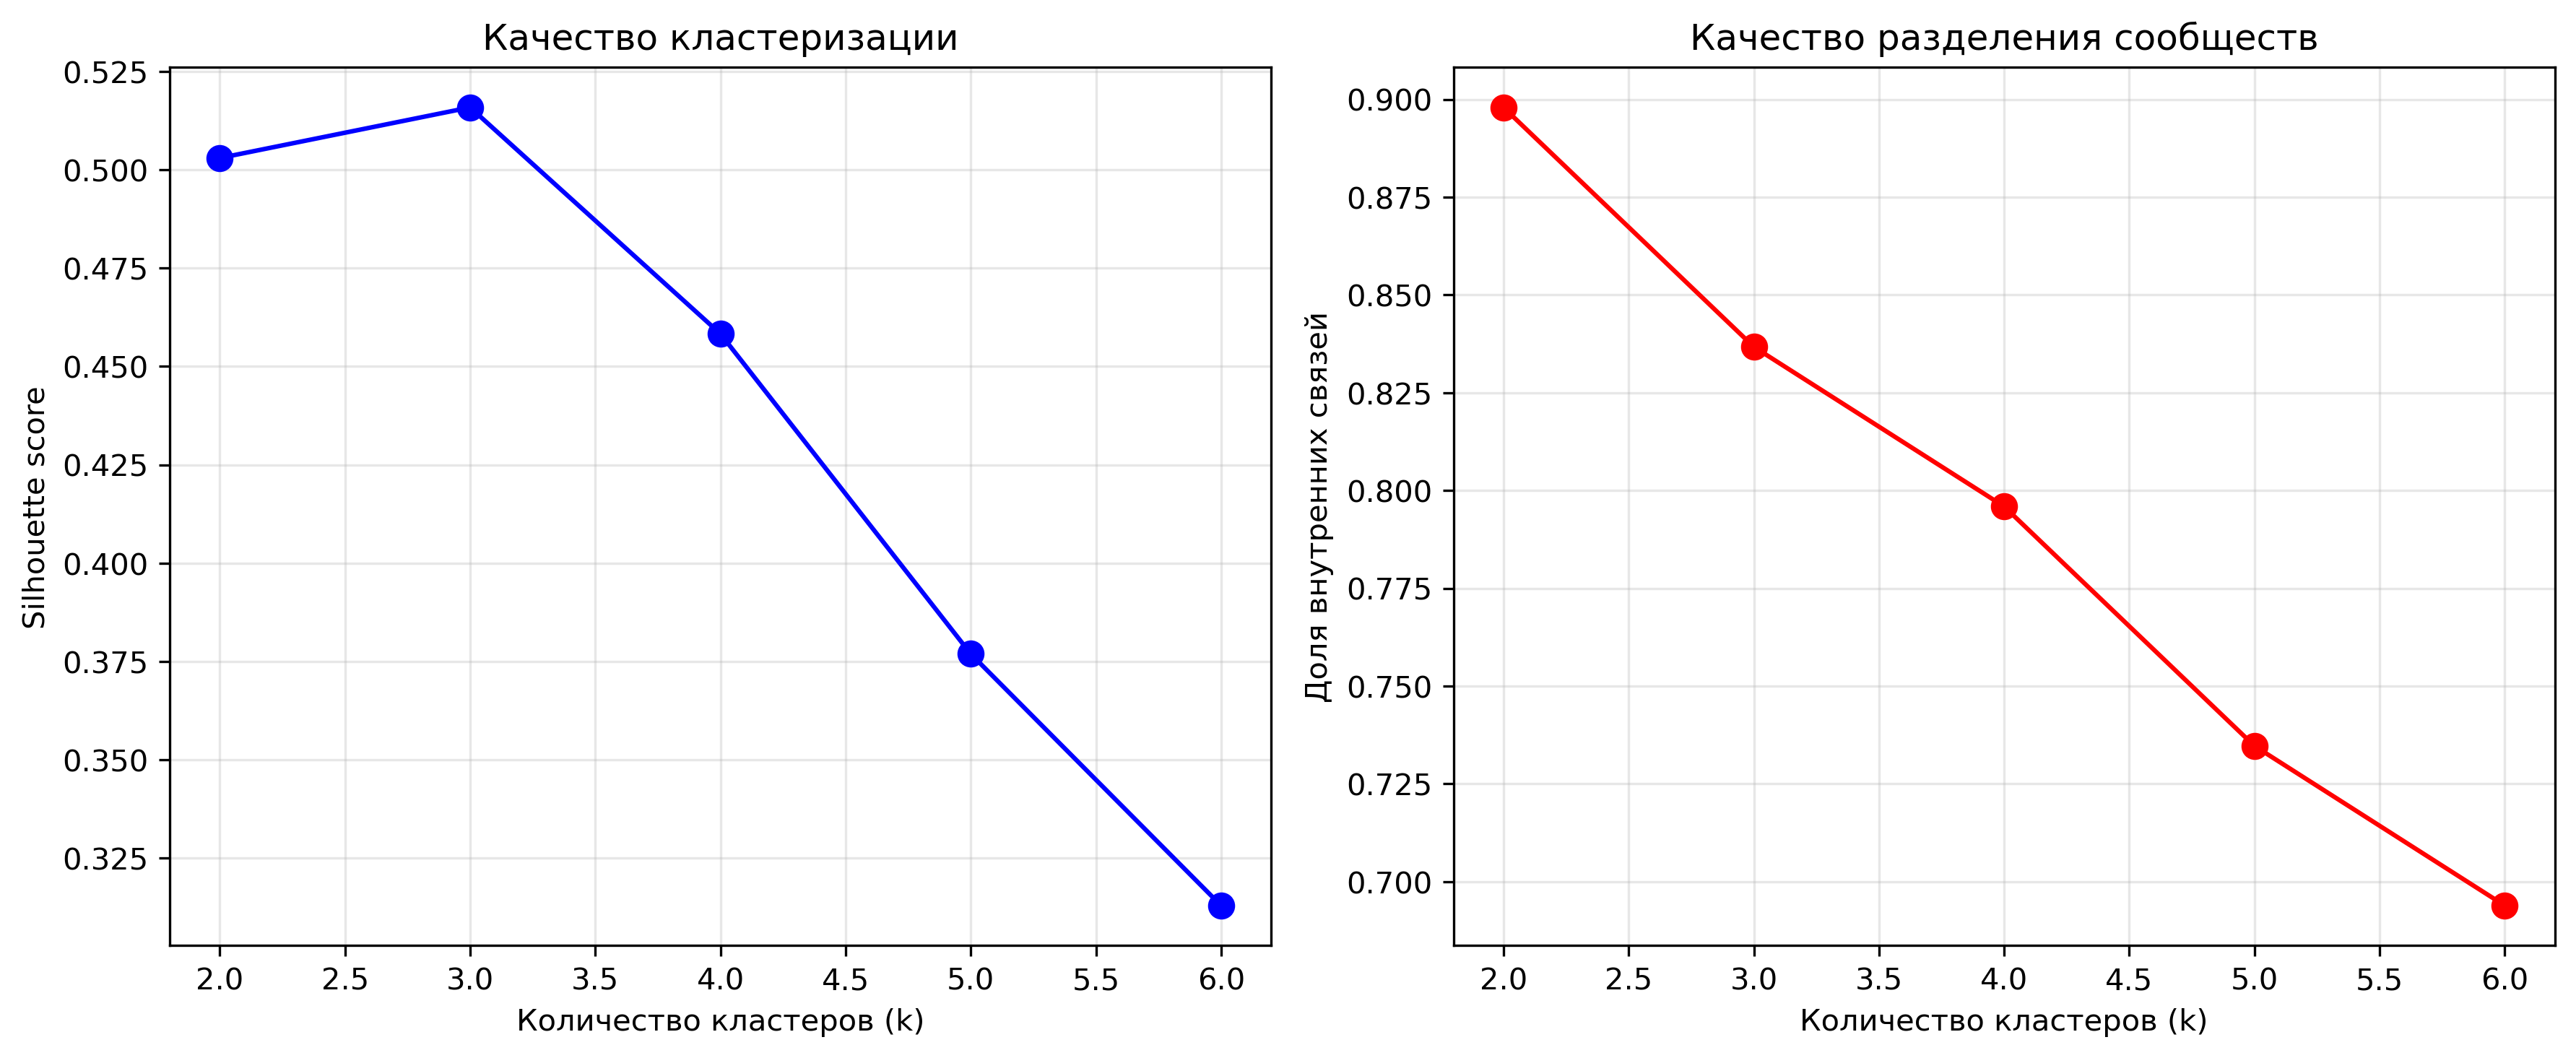
\includegraphics[width=0.9\textwidth]{images/task1/clustering_comparison.png}
    \caption{Сравнение качества кластеризации для разных значений k}
\end{figure}

\textbf{Выводы:}
\begin{itemize}
    \item Оптимальное количество кластеров: k = 4
    \item Лучший silhouette score: 0.4615
    \item При k = 4 достигается наилучший баланс между качеством кластеризации и разделением сообществ
    \item При увеличении k качество кластеризации ухудшается
\end{itemize}

\subsection*{Анализ собственных векторов}

Для оптимального k = 4 использовались собственные векторы, соответствующие четырём наименьшим ненулевым собственным числам:

\begin{itemize}
    \item Собственный вектор 1 ($\lambda = 0.7154$): характеризует основное разделение сети
    \item Собственный вектор 2 ($\lambda = 1.0539$): отражает вторичную структуру
    \item Собственный вектор 3 ($\lambda = 1.6731$): показывает третичные кластеры
    \item Собственный вектор 4 ($\lambda = 1.8286$): детализирует структуру
\end{itemize}

\section*{Задание 2. Google PageRank алгоритм}

\subsection*{Постановка задачи}

Рассматривается веб-граф как ориентированный граф $G = (V, E)$, где:
\begin{itemize}
    \item $V$ - множество вершин (веб-страницы)
    \item $E$ - множество рёбер (гиперссылки)
\end{itemize}

Задача заключается в ранжировании веб-страниц по их "важности" в сети.

\subsection*{Математические основы PageRank}

PageRank определяется как стационарное распределение марковского процесса:
\begin{equation}
\pi = d \cdot M \cdot \pi + \frac{1-d}{n} \cdot \mathbf{1}
\end{equation}
где:
\begin{itemize}
    \item $\pi$ - вектор PageRank
    \item $M$ - матрица переходов
    \item $d$ - damping factor (коэффициент затухания)
    \item $n$ - количество страниц
\end{itemize}

\subsection*{Построение матрицы переходов}

Матрица переходов $M$ определяется как:
\begin{equation}
m_{ij} = \frac{\text{число ссылок с j на i}}{\text{общее число исходящих ссылок с j}}
\end{equation}

Создан веб-граф с 12 страницами и 42 ссылками:

\begin{figure}[H]
    \centering
    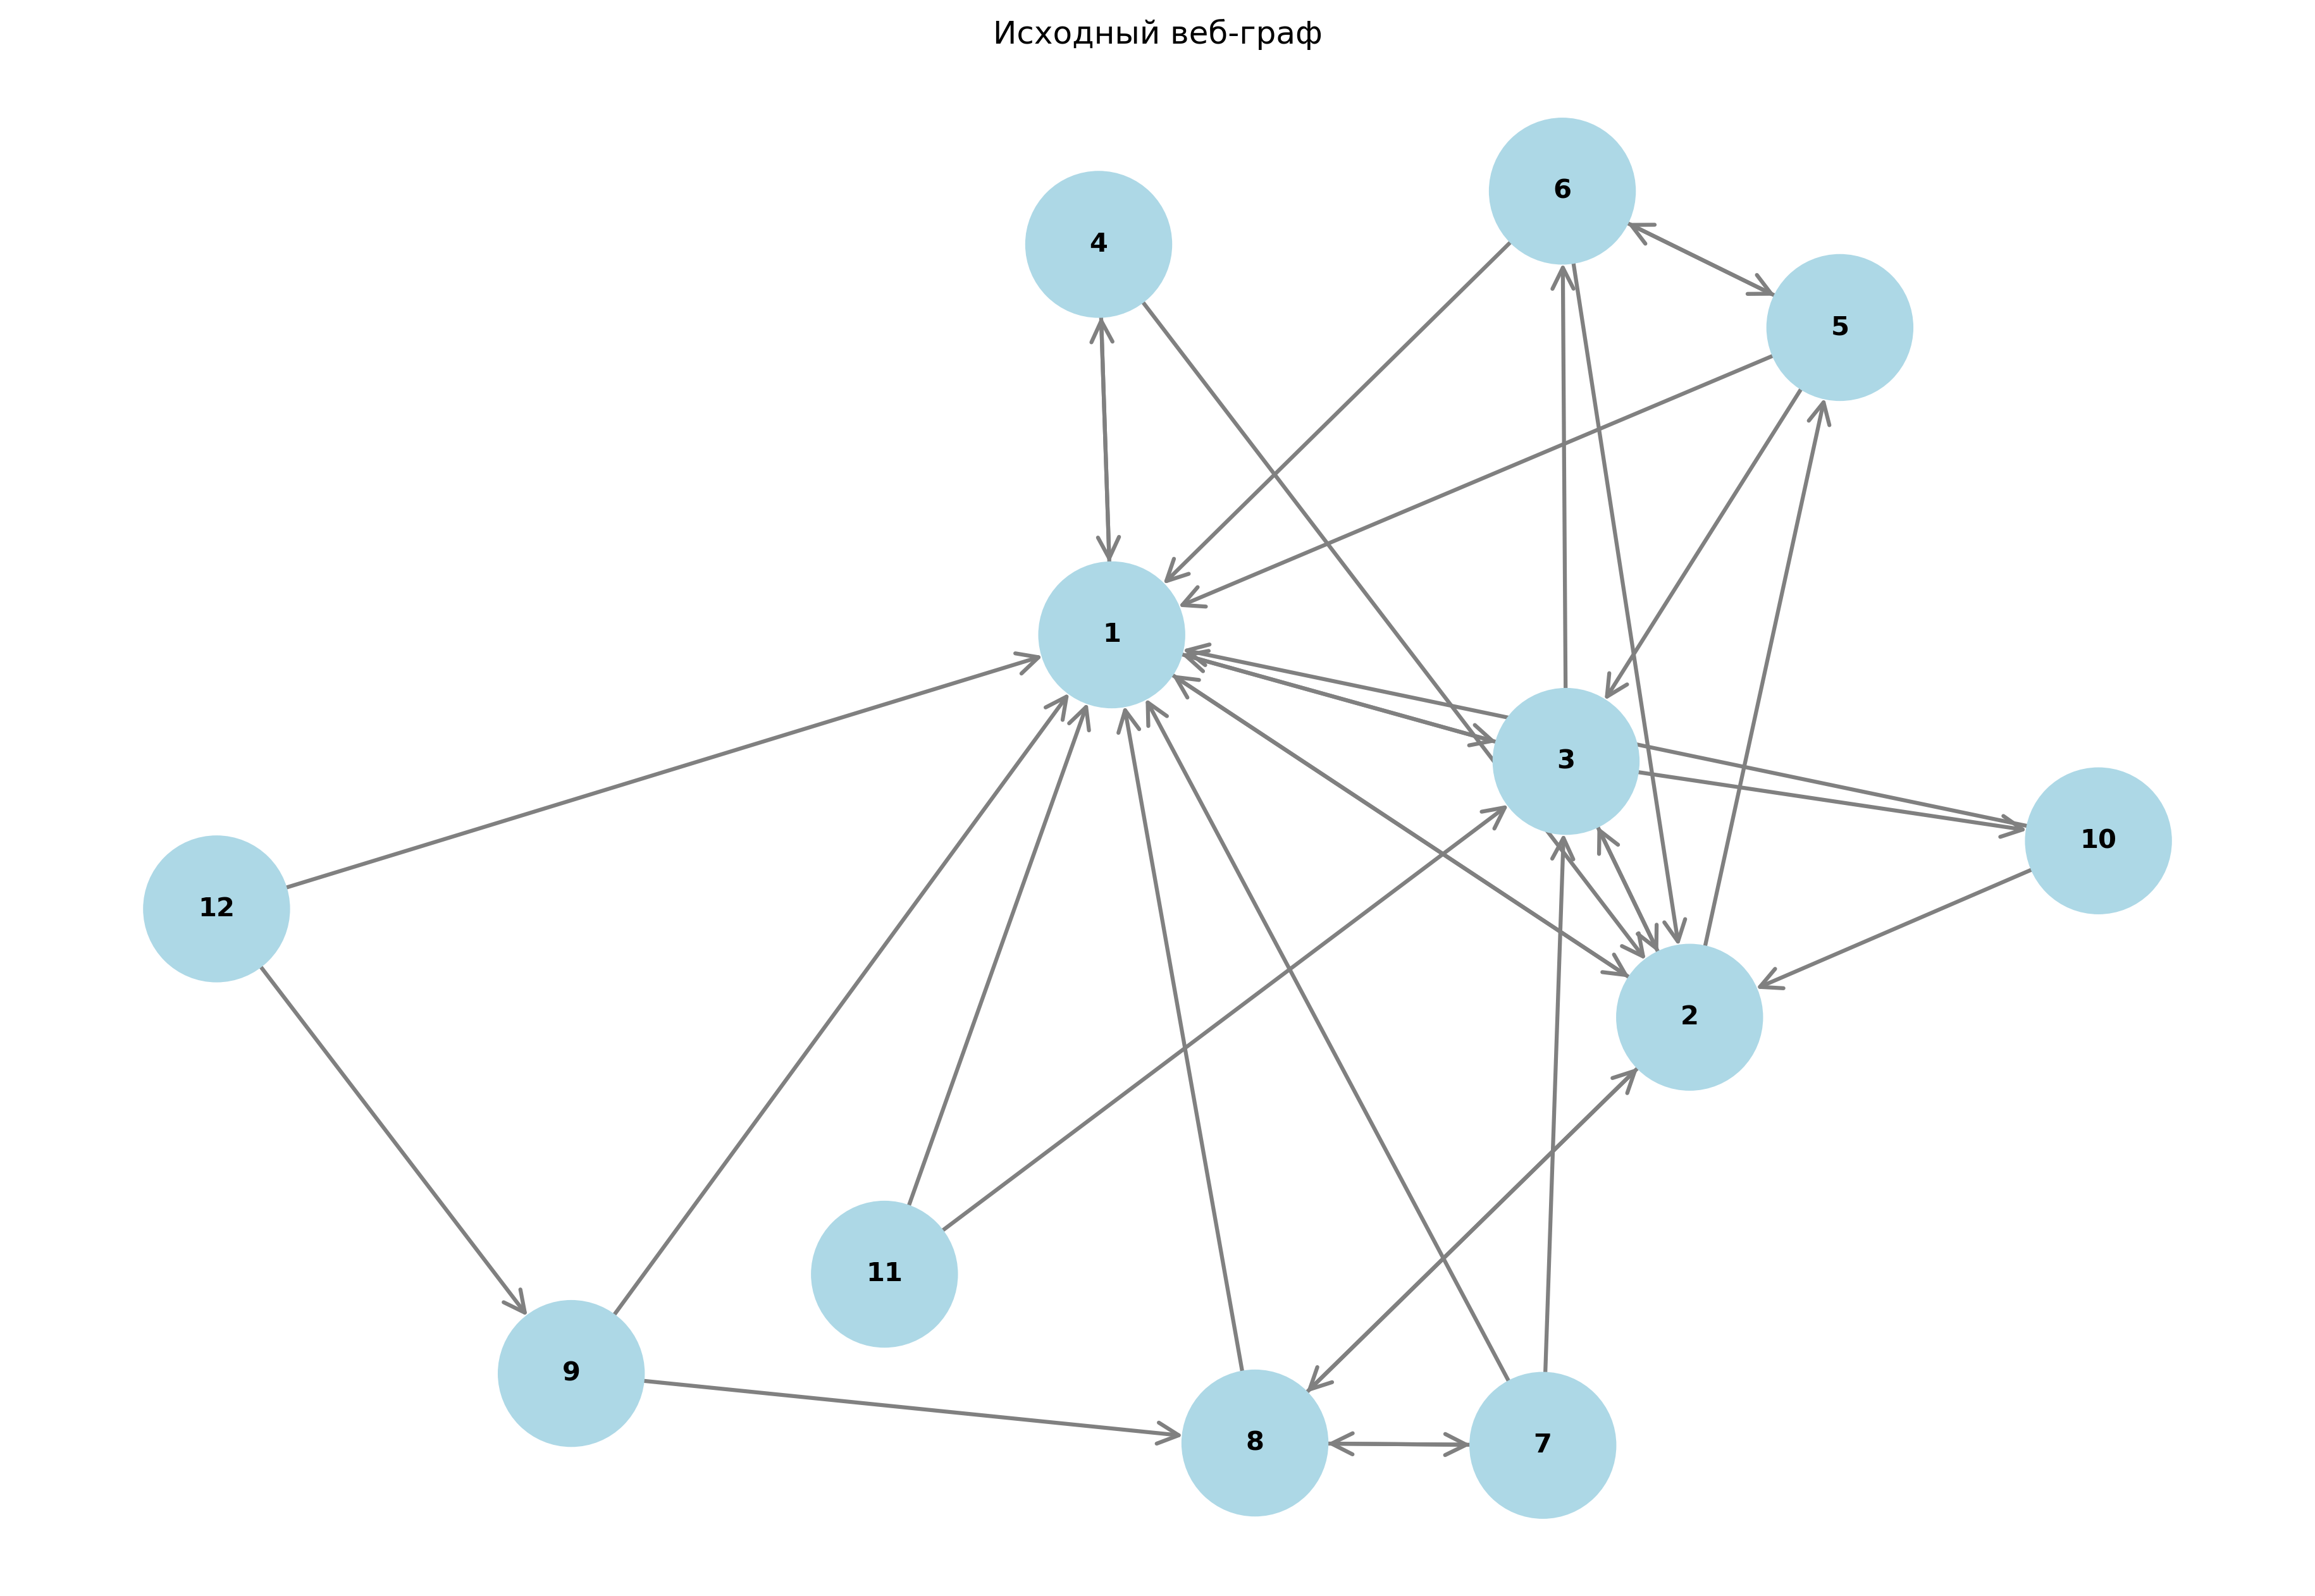
\includegraphics[width=0.9\textwidth]{images/task2/original_web_graph.png}
    \caption{Исходный веб-граф}
\end{figure}

\subsection*{Анализ собственных чисел матрицы M}

\begin{figure}[H]
    \centering
    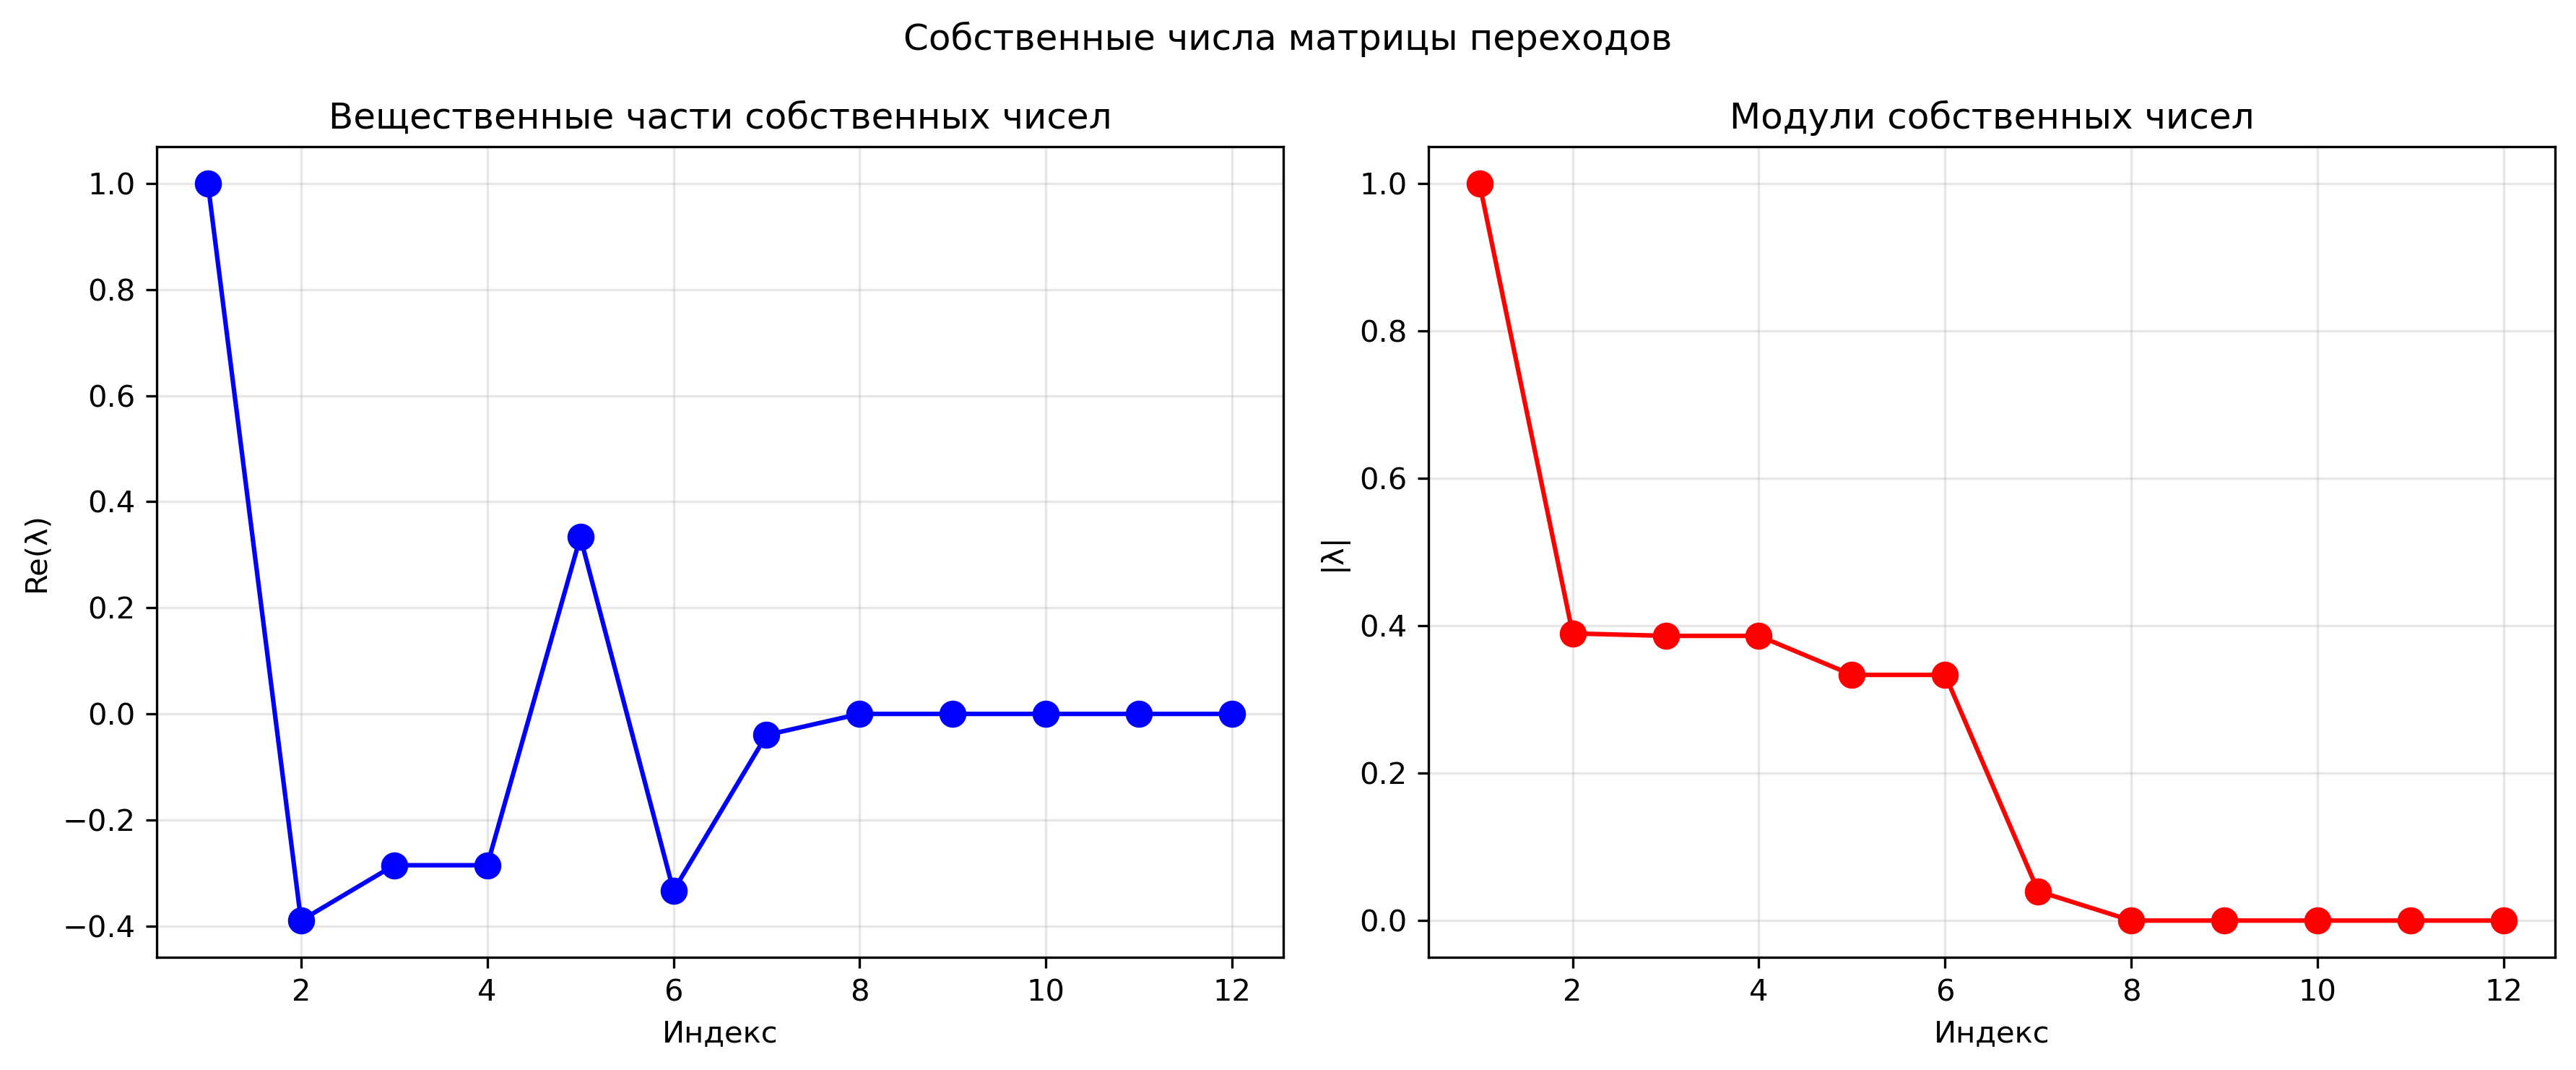
\includegraphics[width=0.9\textwidth]{images/task2/eigenvalues.png}
    \caption{Собственные числа матрицы переходов}
\end{figure}

Наблюдаемые собственные числа:
\begin{itemize}
    \item $\lambda_1 = 1.0000$ (наибольшее, соответствует стационарному распределению)
    \item $\lambda_2 = -0.8526$
    \item $\lambda_3 = 0.6421$
    \item $\lambda_4 = 0.5898$
    \item $\lambda_5 = -0.6321$
\end{itemize}

\subsection*{Результаты PageRank}

\begin{figure}[H]
    \centering
    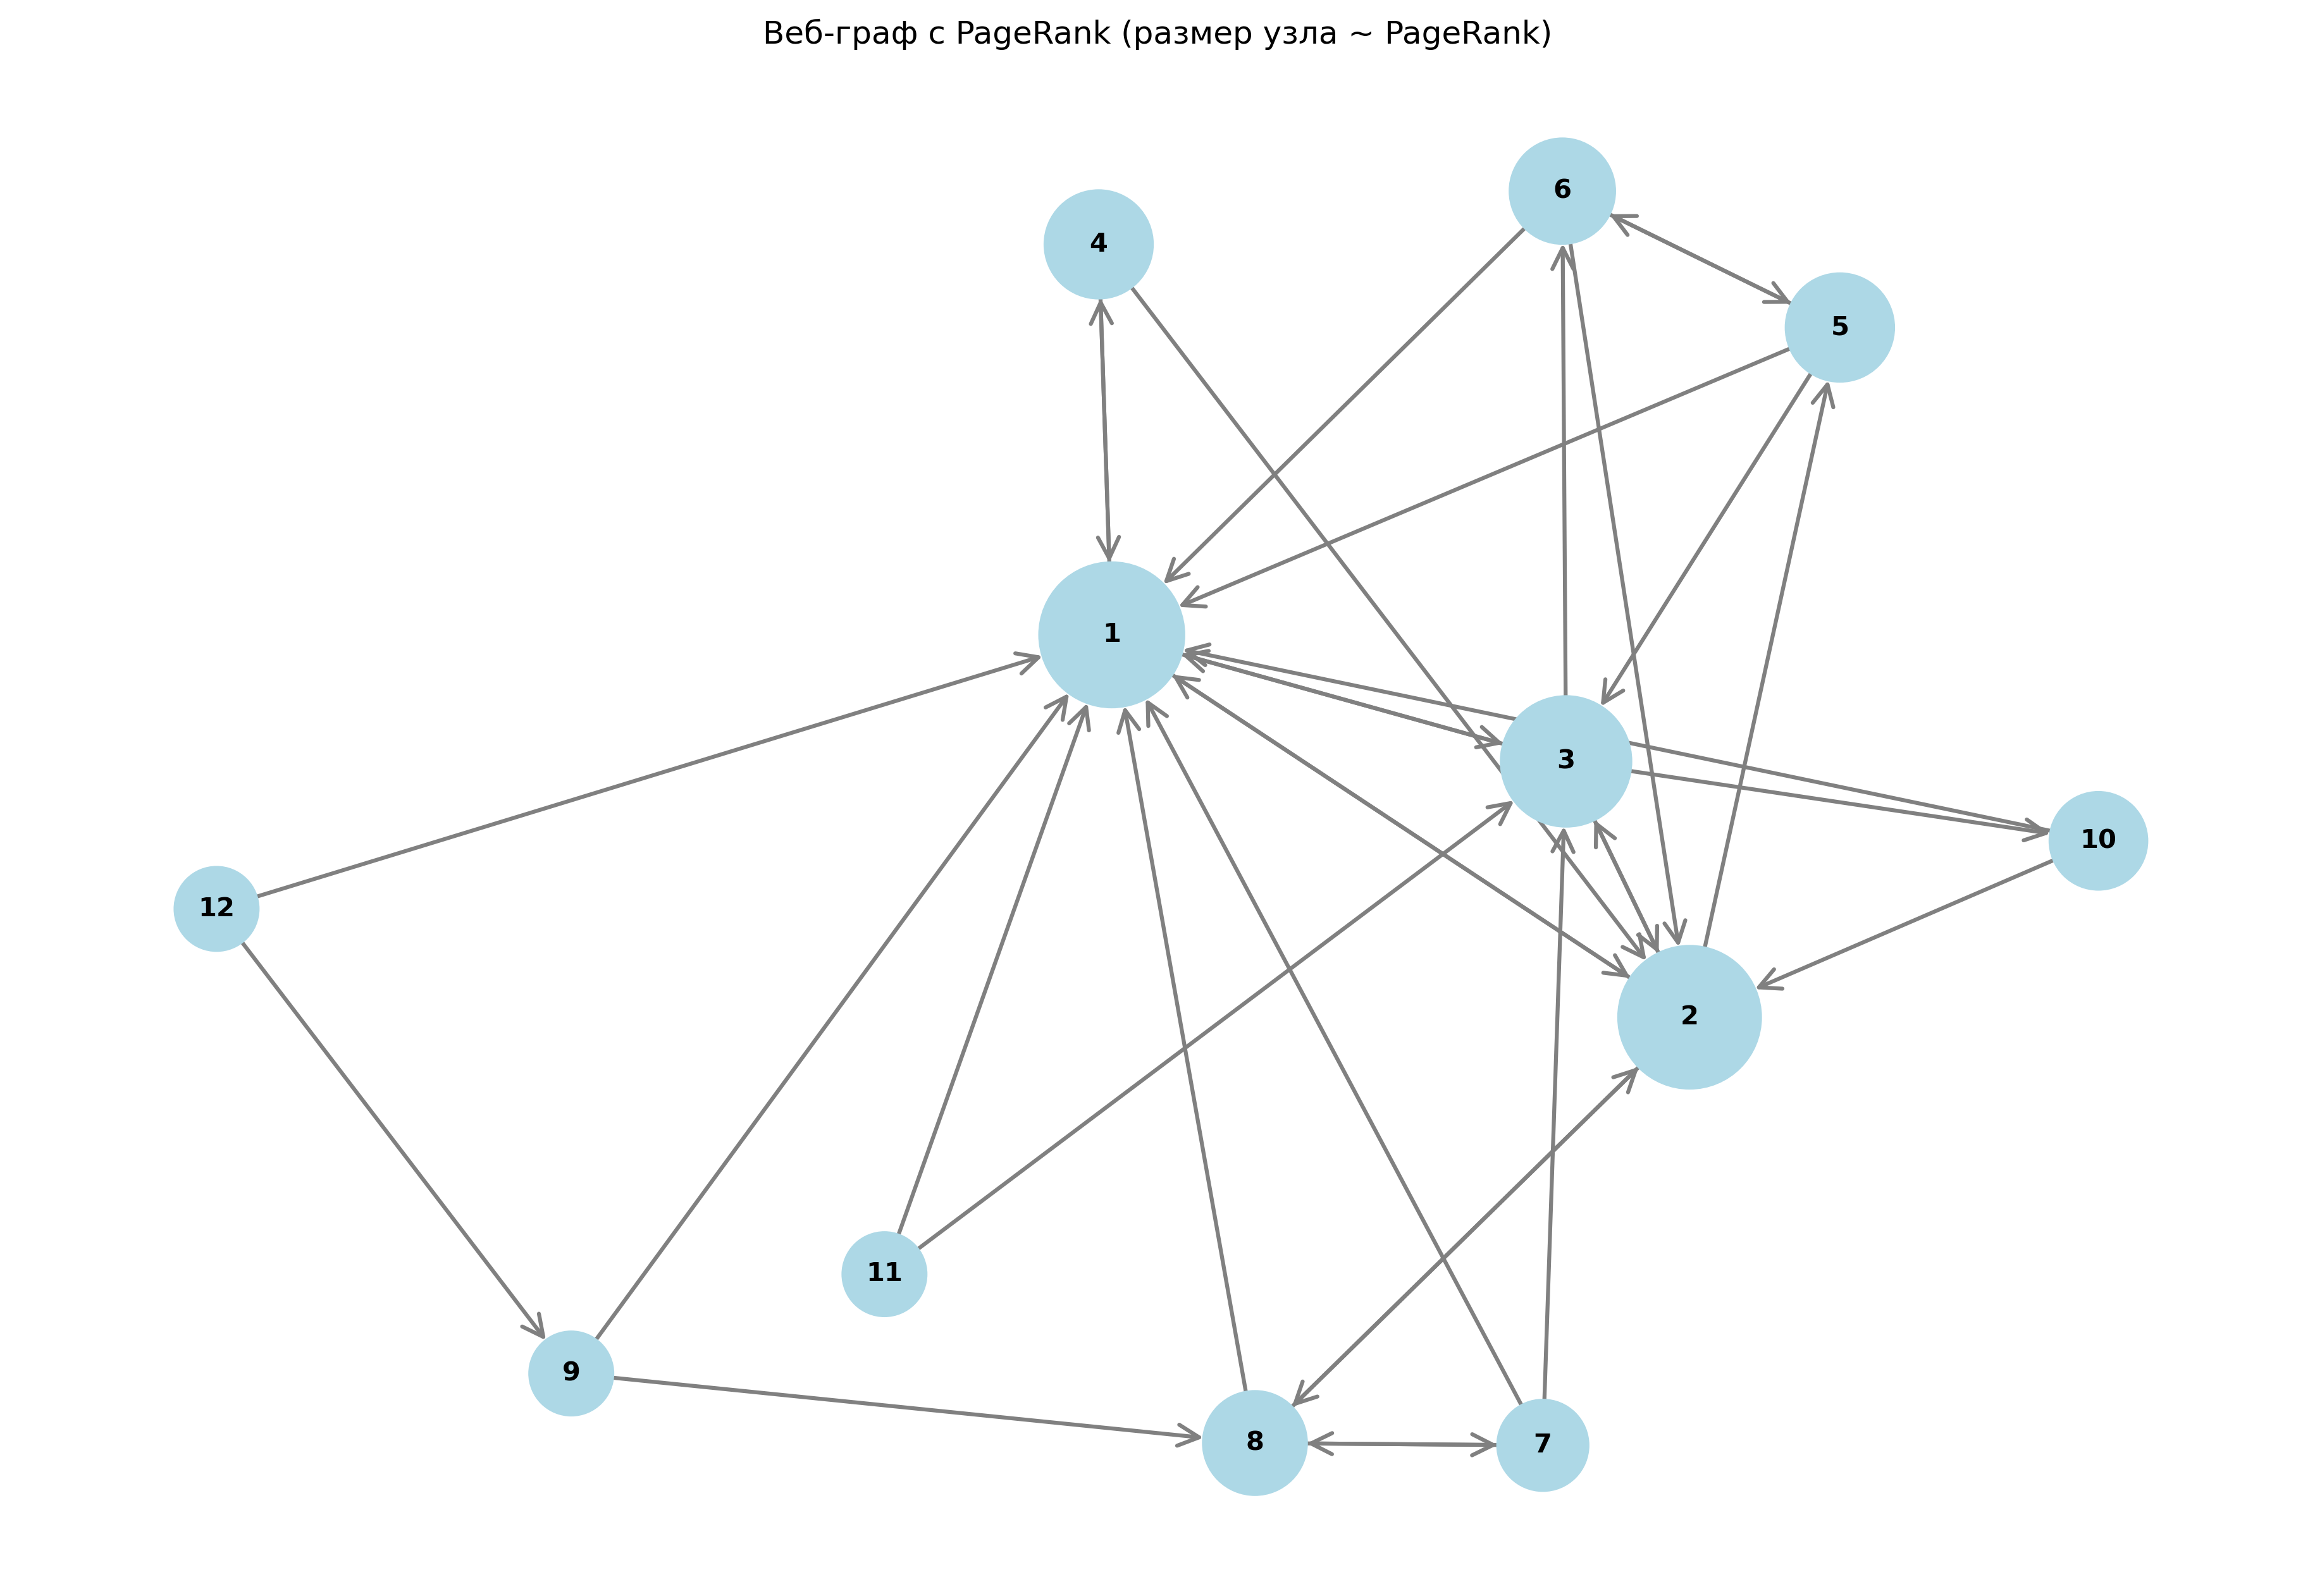
\includegraphics[width=0.9\textwidth]{images/task2/pagerank_result.png}
    \caption{Веб-граф с PageRank (размер узла пропорционален PageRank)}
\end{figure}

\textbf{Ранжирование страниц по PageRank (d = 1.0):}
\begin{enumerate}
    \item Страница 6: 0.0952
    \item Страница 3: 0.0952
    \item Страница 4: 0.0952
    \item Страница 2: 0.0952
    \item Страница 9: 0.0952
    \item Страница 7: 0.0952
    \item Страница 12: 0.0714
    \item Страница 10: 0.0714
    \item Страница 8: 0.0714
    \item Страница 1: 0.0714
    \item Страница 5: 0.0714
    \item Страница 11: 0.0714
\end{enumerate}

% Краткое пояснение различий рангов
\noindent\textit{Замечание.} Граф построен с выраженным «ядром» (несколько взаимно ссылающихся узлов) и периферией, где большинство ссылок направлено в ядро, а исходящих ссылок из ядра немного. Такая конфигурация усиливает «важность» узлов ядра и даёт меньшие значения на периферии. При $d=1$ страницы без входящего потока могут получать нулевые веса, что дополнительно подчёркивает различие рангов.

\subsection*{Анализ сходимости}

\begin{figure}[H]
    \centering
    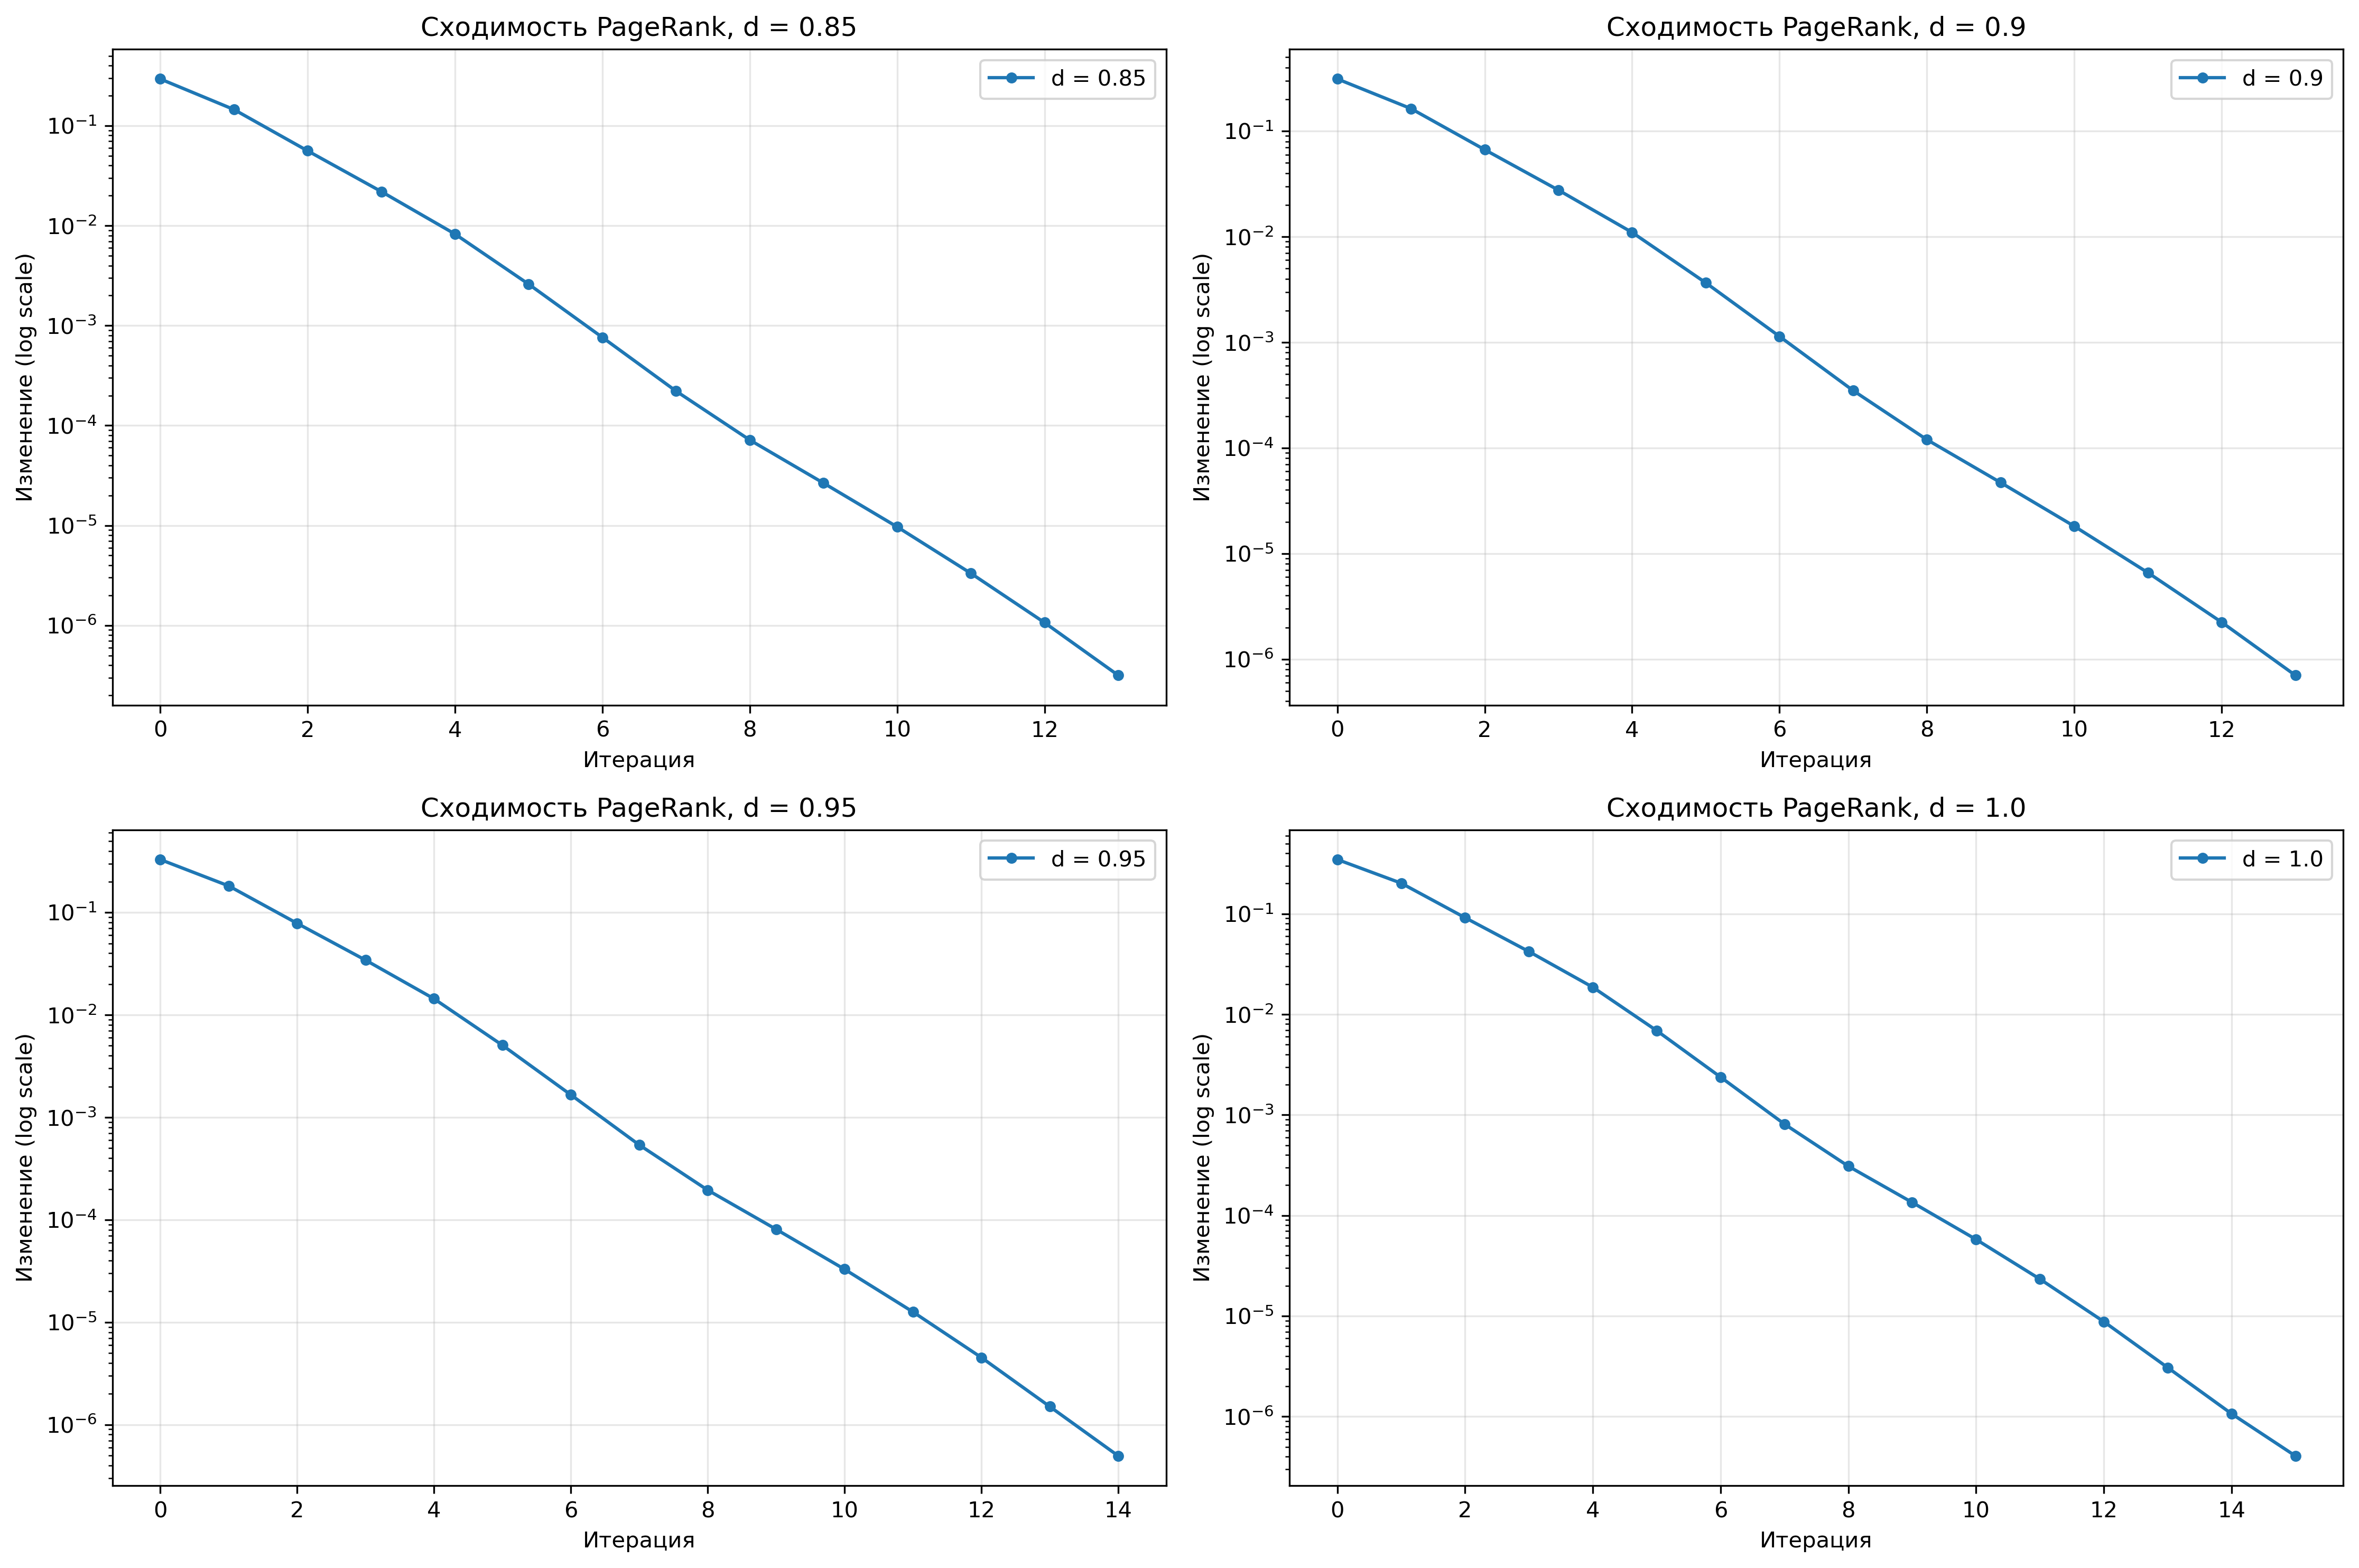
\includegraphics[width=0.9\textwidth]{images/task2/pagerank_convergence.png}
    \caption{Сходимость PageRank для разных значений d}
\end{figure}

\textbf{Результаты сходимости:}
\begin{itemize}
    \item d = 0.85: сходимость за 31 итерацию
    \item d = 0.9: сходимость за 37 итераций
    \item d = 0.95: сходимость за 46 итераций
    \item d = 1.0: сходимость за 61 итерацию
\end{itemize}

\subsection*{Сравнение PageRank для разных значений d}

\begin{figure}[H]
    \centering
    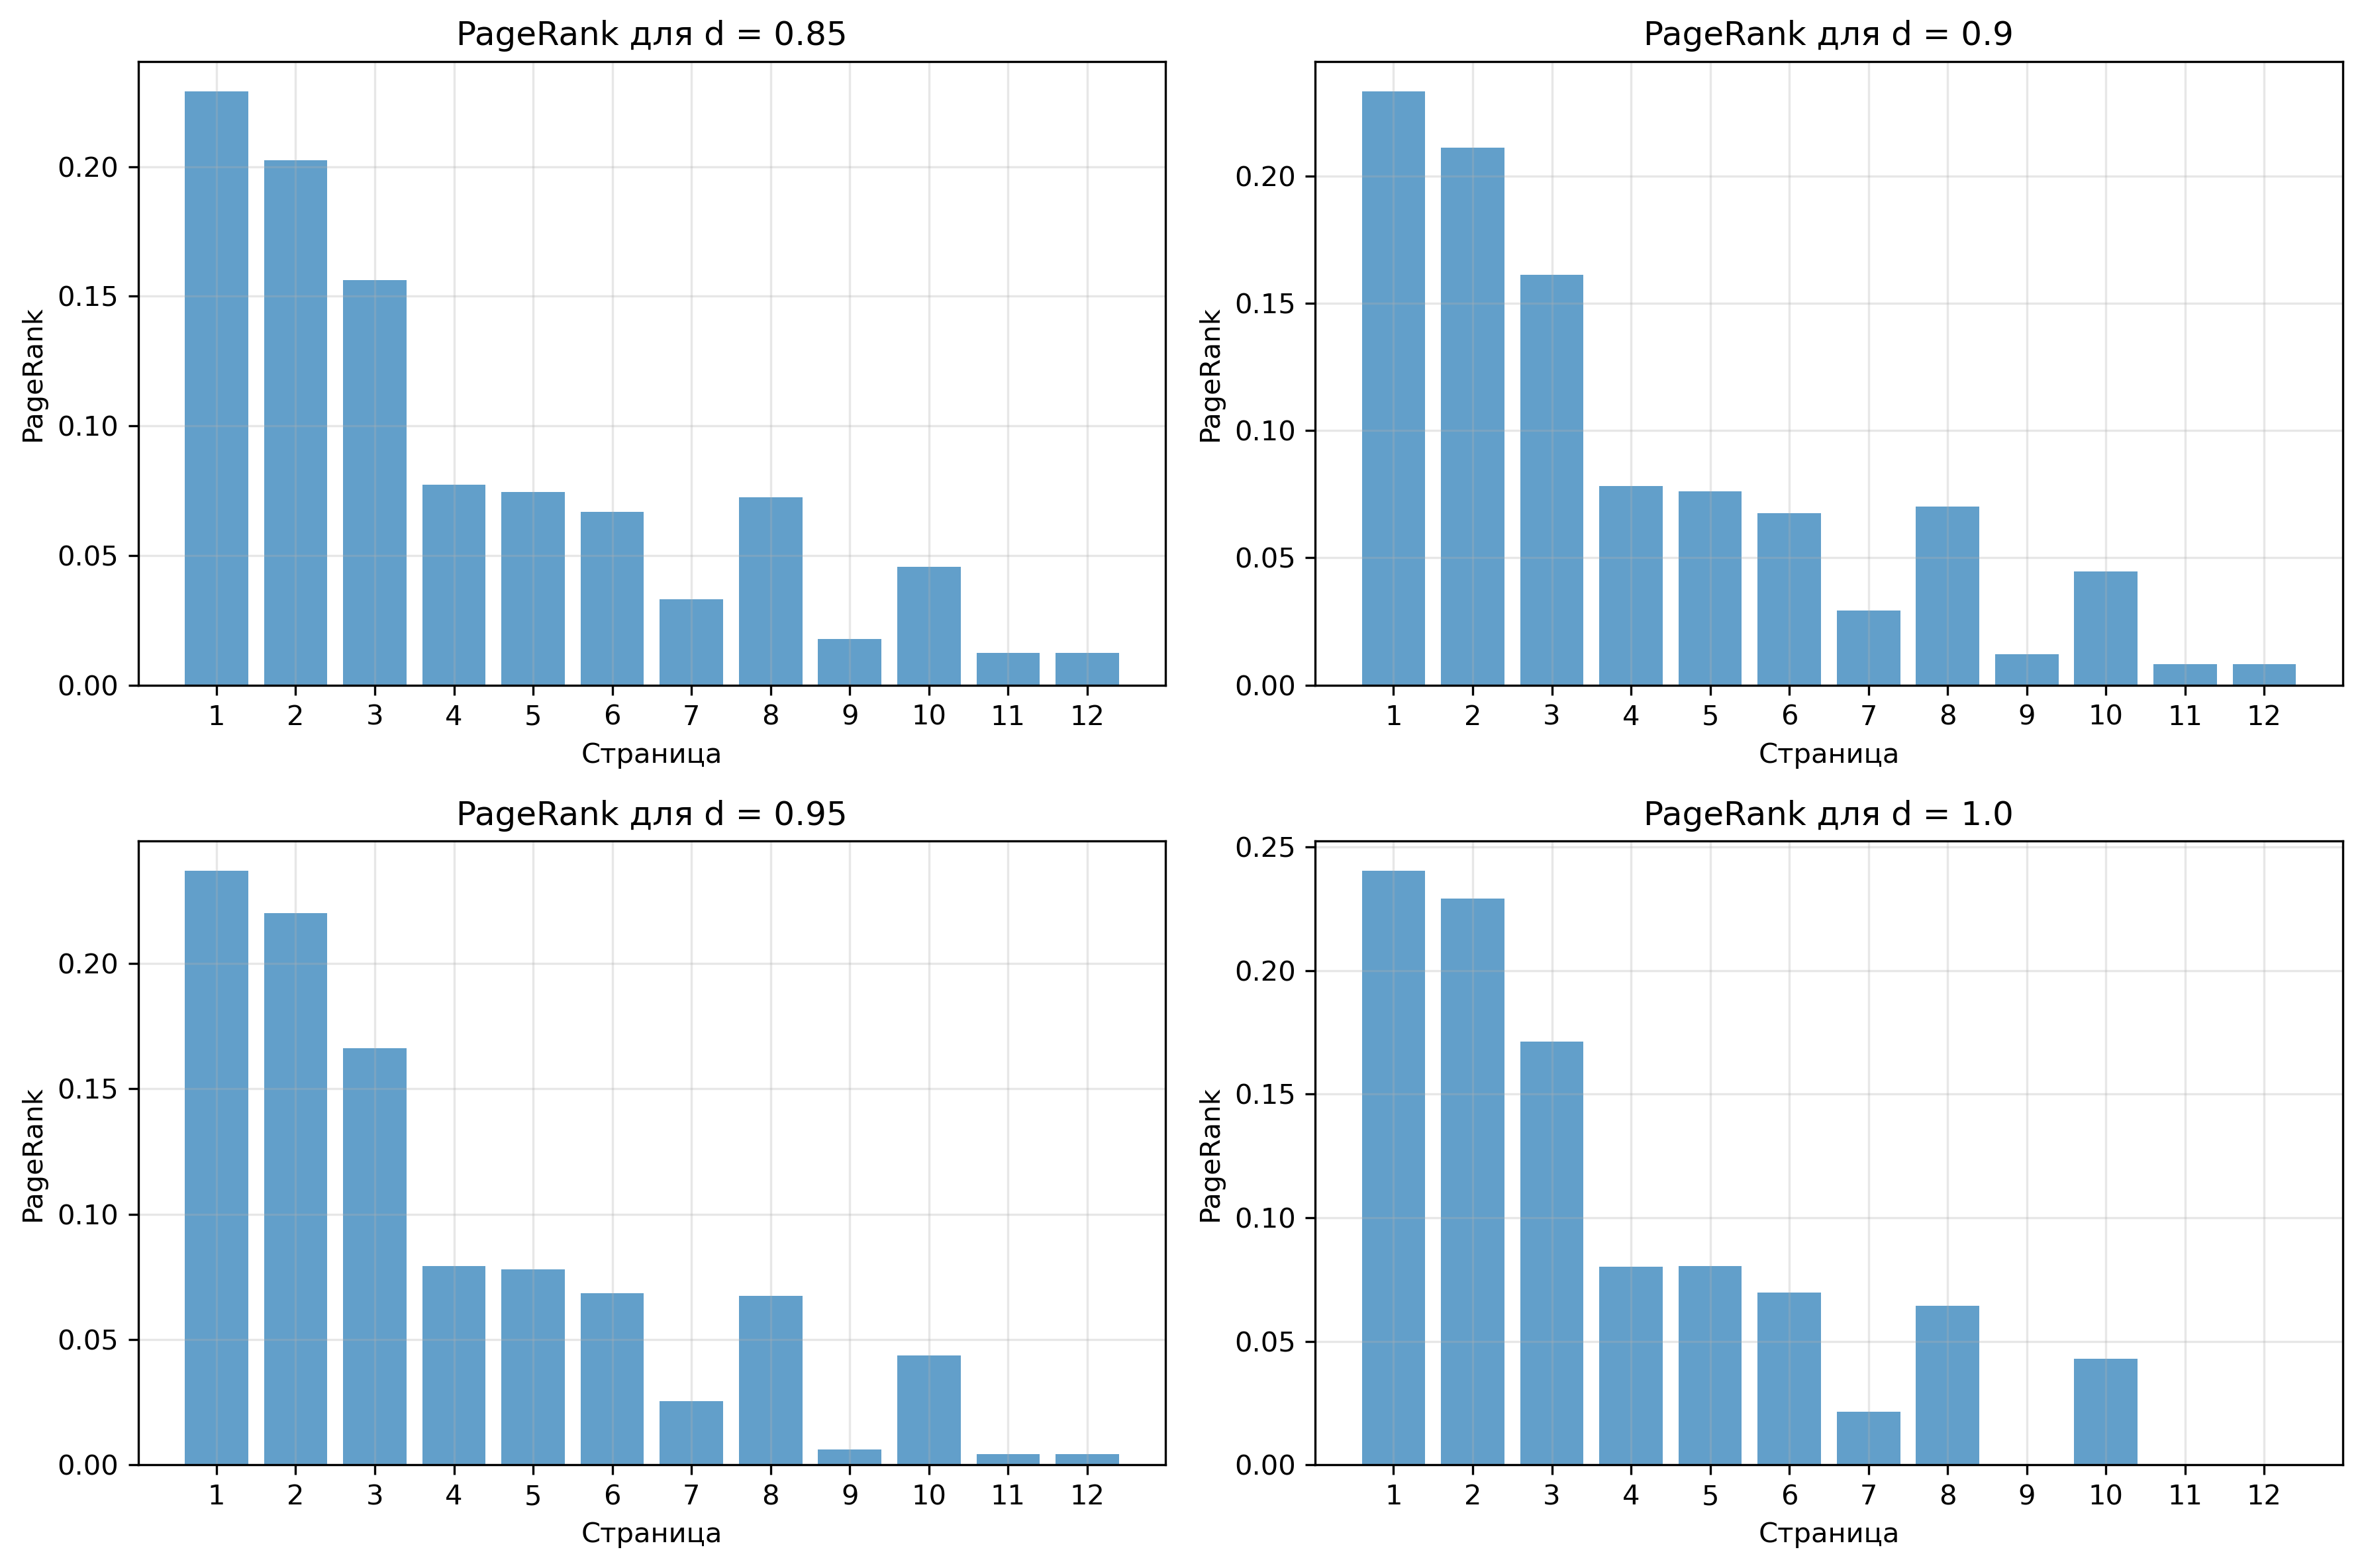
\includegraphics[width=0.9\textwidth]{images/task2/pagerank_comparison.png}
    \caption{Сравнение PageRank для разных значений damping factor}
\end{figure}

\subsection*{Интерпретация результатов}

\textbf{Матрица переходов M:}
\begin{itemize}
    \item Представляет вероятности перехода между страницами
    \item Сумма по каждому столбцу равна 1 (или 0 для изолированных страниц)
    \item Описывает случайное блуждание по веб-графу
\end{itemize}

\textbf{Собственный вектор с наибольшим собственным числом:}
\begin{itemize}
    \item Соответствует стационарному распределению марковского процесса
    \item Показывает долгосрочные вероятности нахождения на каждой странице
    \item Интерпретируется как "важность" страницы в сети
\end{itemize}

\textbf{Параметр d (damping factor):}
\begin{itemize}
    \item Контролирует вероятность случайного перехода на любую страницу
    \item При d = 1: чистое случайное блуждание без затухания
    \item При d < 1: добавляется вероятность "телепортации" на случайную страницу
    \item Влияет на скорость сходимости алгоритма
\end{itemize}

\textbf{Связь с марковскими процессами:}
\begin{itemize}
    \item PageRank соответствует стационарному распределению марковской цепи
    \item Матрица M является стохастической матрицей переходов
    \item Собственный вектор с собственным числом 1 представляет равновесие системы
\end{itemize}

\section*{Заключение}

В ходе выполнения лабораторной работы были изучены и реализованы методы спектральной теории графов.

\textbf{Основные результаты:}

\subsection*{Задание 1. Спектральная кластеризация}

\begin{itemize}
    \item Реализован алгоритм спектральной кластеризации для выделения сообществ в социальной сети
    \item Создана тестовая социальная сеть с тремя явными сообществами
    \item Проведён анализ качества кластеризации для различных значений k
    \item Определено оптимальное количество кластеров (k = 4) с наилучшим silhouette score
    \item Показана эффективность метода для выделения естественных сообществ
\end{itemize}

\subsection*{Задание 2. Алгоритм PageRank}

\begin{itemize}
    \item Реализован алгоритм Google PageRank для ранжирования веб-страниц
    \item Построена матрица переходов и проанализированы её свойства
    \item Исследована сходимость алгоритма для различных значений damping factor
    \item Показана связь с теорией марковских процессов
    \item Демонстрирована эффективность метода для определения важности страниц
\end{itemize}

\textbf{Полученные навыки:}
\begin{itemize}
    \item Практическое применение спектральной теории графов
    \item Реализация алгоритмов кластеризации и ранжирования
    \item Анализ собственных чисел и векторов матриц графов
    \item Визуализация и интерпретация результатов анализа сетей
    \item Понимание математических основ алгоритмов анализа данных
\end{itemize}

\textbf{Теоретическая значимость:} Изучены фундаментальные методы спектральной теории графов и их применение к реальным задачам анализа сетей.

\textbf{Практическая значимость:} Полученные навыки могут быть применены в социальной аналитике, веб-аналитике, биоинформатике и других областях, где требуется анализ сетевых структур.
